\documentclass[a4paper]{book} %{article}

\usepackage{fullpage} % Package to use full page
\usepackage{parskip} % Package to tweak paragraph skipping
\usepackage{tikz} % Package for drawing
\usepackage{amsmath}
\usepackage{hyperref}
\usepackage[numbered]{bookmark} % For numbering of challenges in bookmark pane of PDF viewer
\def\UrlBreaks{\do\/\do-}
\usepackage[absolute]{textpos}
\setlength{\TPHorizModule}{1mm}
\setlength{\TPVertModule}{1mm}
\usepackage{tikz}
\usepackage{siunitx}
\usepackage{datetime} % Time
\usepackage[UKenglish]{isodate}
\usepackage{ctable} % Thick table lines
\usepackage{booktabs} % Merge cells with multicolumn
\usepackage{bm} % Bold-maths \bm command
\usepackage{pdfpages} % Insert PDF into PDF

\newcommand{\courseyear}{2018 }
\newcommand{\disctime}{08:40 to 10:10 }
\newcommand{\discdays}{Mondays }
\newcommand{\discroom}{Centre Zone 1409}
\newcommand{\course}{Ordinary Differential Equations }
\newcommand{\courseurl}{ordinary-differential-equations}
\newcommand{\nensei}{2nd}

\newcommand{\lap}[1]{\mathcal{L}\{#1\}}

\newcommand{\six}[1]{\SI[parse-numbers=false]{X}{#1}}
\newcommand{\hash}[2]{MD5(#1\_X) = #2\ldots}
\newcommand{\timebox}{\vfill Study-time (from end of previous challenge to end of this challenge): \underline{\hspace{1cm} minutes}}
\newcommand{\matrixcrr}[2]{\left(\begin{array}{c}{#1}\\{#2}\end{array}\right)}
\newcommand{\matrixccrr}[4]{\left(\begin{array}{cc}{#1}&{#2}\\{#3}&{#4}\end{array}\right)}

\newcommand{\solint}[2]{X = Your solution\\Form: Integer.\\Place the indicated letter in front of the number.\\Example: aX where $X=46$ is entered as \href{http://www.wolframalpha.com/input/?i=md5+hash+of+\%22a46\%22}{a46}\\\\Hash of {#1}X = {#2}}
\newcommand{\soltwodp}[2]{X = Your solution\\Form: Decimal to 2 decimal places.\\Place the indicated letter in front of the number.\\Example: aX where $X=46.00$ is entered as \href{http://www.wolframalpha.com/input/?i=md5+hash+of+\%22a46.00\%22}{a46.00}\\\\Hash of {#1}X = {#2}}
\newcommand{\solstr}[2]{X = Your solution\\Form: String.\\Place the indicated letter in front of the string.\\Example: aX where $X=\text{abcdef}$ is entered as \href{http://www.wolframalpha.com/input/?i=md5+hash+of+\%22a46.00\%22}{aabcdef}\\\\Hash of {#1}X = {#2}}

\graphicspath{{Images/}}

\begin{document}

\begin{titlepage}
    \begin{center}
        \vspace*{1cm}

        \Huge
        \textbf{Ordinary Differential Equations}

        Autumn \courseyear

        \vspace{1.5cm}
        \Large
        Last updated:\\\today \ at \currenttime

        \vspace{4.0cm}
        \LARGE
        James Cannon\\Kyushu University
        \vfill

        \normalsize
        \url{http://www.jamescannon.net/teaching/\courseurl}\\
        \vspace{0.3cm}
        \small
        \url{http://raw.githubusercontent.com/NanoScaleDesign/OrdinaryDifferentialEquations/master/ode.pdf}
        \vspace{0.5cm}

        License: \emph{CC BY-NC 4.0}.

    \end{center}
\end{titlepage}

\setcounter{chapter}{-1}

\tableofcontents

\chapter{Course information}
\newpage
\section{This course}
This course is the \course course studied at Kyushu University by \nensei-year students.

\subsection{How this works}
\begin{itemize}
    \item In contrast to the traditional lecture-homework model, in this course the learning is self-directed and active via publicly-available resources.
    \item Learning is guided through solving a series of carefully-developed challenges contained in this book (download from \url{http://www.jamescannon.net/teaching/\courseurl}), coupled with suggested resources that can be used to solve the challenges with instant feedback about the correctness of your answer.
    \item There are no lectures. Instead, there is discussion time. Here, you are encouraged to discuss any issues with your peers, teacher and any teaching assistants. Furthermore, you are encouraged to help your peers who are having trouble understanding something that you have understood; by doing so you actually increase your own understanding too.
    \item Peer discussion is encouraged, however, if you have help to solve a challenge, always make sure you do understand the details yourself. You will need to be able to do this in an exam environment. If you need additional challenges to solidify your understanding, then ask the teacher. The questions on the exam will be similar in nature to the challenges. If you can do all of the challenges, you can get 100\% on the exam.
    \item Discussion-time is from \disctime on \discdays at room \discroom.
    \item Every challenge in the book typically contains a \textbf{Challenge} with suggested \textbf{Resources} which you are recommended to utilise in order to solve the challenge. A \textbf{Solution} is made available in encrypted form. If your encrypted solution matches the encrypted solution given, then you know you have the correct answer and can move on. For more information about encryption, see section \ref{sec:hashes}. Occasionally the teacher will provide extra \textbf{Comments} to help guide your thinking.
    \item For deep understanding, it is recommended to study the suggested resources beyond the minimum required to complete the challenge.
    \item The challenge document has many pages and is continuously being developed. Therefore it is advised to view the document on an electronic device rather than print it. The date on the front page denotes the version of the document. You will be notified by email when the document is updated.
    \item A “target challenge” and “minimum challenge” will be set each week, to be achieved by the beginning of the discussion time.
    \begin{itemize}
        \item Target challenge: You are expected to complete at least up to this challenge. This is because the “group learning” effect is strongest when everyone is roughly around the same level of understanding.
        \item Minimum challenge: Due to personal (eg health) or professional (eg conference attendance) issues, or simply difficulties with the challenges, it may occasionally not be possible to reach the target challenge. In this case, you will still be considered to be progressing normally if you achieve the minimum challenge.
        \item You may work ahead, even beyond the target challenge, if you so wish. This can build greater flexibility into your personal schedule, especially as you become busier towards the end of the semester.
    \end{itemize}
    \item Your contributions to the course are strongly welcomed. If you come across resources that you found useful that were not listed by the teacher or points of friction that made solving a challenge difficult (there's no such thing as ``you should have learned it in high-school'' - you're probably not the only one with that specific problem), please let the teacher know about it!
\end{itemize}

\subsection{Assessment}
In order to prove to outside parties that you have learned something from the course, we must perform summative assessments. This will be in the form of
\begin{itemize}
    \item Exam(s): Final exam, and possibly a mid-term exam
    \item Group presentation towards the end of the course (details to be announced later)
\end{itemize}

\subsection{What you need to do}
\begin{itemize}
    \item Prepare a challenge-log in the form of a workbook or folder where you can clearly write the calculations you perform to solve each challenge. This will be a log of your progress during the course and will be occasionally reviewed by the teacher.
    \item You will need to maintain a google spreadsheet detailing your work and progress. The purpose of this spreadsheet is to help the teacher optimise the discussion-time. Please ensure that it is up-to-date 24 hours before each discussion-time starts. It is fine for you to continue to work on challenges and update the spreadsheet after the 24-hour deadline.
    \item You also need to submit a brief report at \url{https://goo.gl/forms/Djl4FEZcJLMpipsY2} 24 hours before the discussion time starts. Here you can let the teacher know about any difficulties you are having and if you would like to discuss anything in particular.
    \item Please bring a wifi-capable internet device to class, as well as headphones if you need to access online components of the course during class. If you let me know in advance, I can lend computers and provide power extension cables for those who require them (limited number).
\end{itemize}

\subsection{Details about the spreadsheet}
To get started:
\begin{enumerate}
    \item Log into google
    \item Open \url{http://bit.ly/2cPYyQY}
    \item File $\rightarrow$ Make a copy [$\rightarrow$ rename] $\rightarrow$ ok
    \item Click ``Share'' (top right)
    \item Click ``Get shareable link''
    \item Set ``Anyone with the link can view''
    \item Copy sharing address
    \item Send an email to cannon@mech.kyushu-u.ac.jp containing
    \begin{enumerate}
       \item Subject: [course name] registration
       \item Your name
       \item Student number
       \item The link to your copy of the google sheet
    \end{enumerate}
\end{enumerate}

Using the spreadsheet:

\begin{itemize}
    \item Enter the appropriate challenge number. For example, for challenge 1.4, enter ``1'' in the \textbf{Section} column and ``4'' in the \textbf{Challenge} column.
    \item After successfully completing a challenge, please enter any particular friction points that you experienced (if any) so the course can be developed to reduce such friction in the future, as well as any extra resources you recommend (if any).
    \item Please also roughly estimate the amount of effort in \textbf{Hours} required to complete the challenge (starting from when you completed the previous challenge, including any reading, watching videos, looking for resources, writing the answer to the challenge, discussing with peers, etc). This is not used for assessment in any way, but is very valuable in helping the teacher develop the course.
\end{itemize}

Note: Please do not alter column names, ordering, etc. Just add section and challenge numbering and fill in the columns as appropriate. This is because spreadsheet data is downloaded and automatically analysed, and it breaks if anything is inconsistent.



\newpage
\section{Timetable}

\begin{center}
    \begin{tabular}{|c|c|c|c|}
        \hline
        & \textbf{Discussion} & \textbf{Target} & \textbf{Note} \\ \specialrule{.1em}{.05em}{.05em}
        \textbf{1}  & 7 Oct  & -            &                          \\ \hline
        \textbf{2}  & 14 Oct & 2.2          &                          \\ \hline
        \textbf{3}  & 21 Oct & 2.7          &                          \\ \hline
        \textbf{4}  & 28 Oct & 2.12         &                          \\ \specialrule{.1em}{.05em}{.05em}
        \textbf{5}  & 4 Nov  & 2.20         &                          \\ \hline
        \textbf{6}  & 11 Nov & 3.8          &                          \\ \hline
        \textbf{7}  & 25 Nov & 3.15         &                          \\ \specialrule{.1em}{.05em}{.05em}
        \textbf{8}  & 2 Dec  & 3.18         & Coursework instructions  \\ \hline                            % Non-homogeneous equations (undetermined coeffs, var of params)
        \textbf{9}  & 9 Dec  & Midterm exam &                          \\ \hline                            % Exam preparation
        \textbf{10} & 16 Dec & 4.6          &                          \\ \specialrule{.1em}{.05em}{.05em}  % Laplace transform
        \textbf{11} & 6 Jan  & 4.12         &                          \\ \hline                            % Laplace transform
        \textbf{12} & 12 Jan & 5.3          & Submission of coursework \\ \hline                            % Systems of differential equations
        \textbf{13} & 20 Jan &              &                          \\ \hline                            % Systems of differential equations
        \textbf{14} & 27 Jan &              &                          \\ \specialrule{.1em}{.05em}{.05em}  % Series
        \textbf{15} & 10 Feb & Final exam   & Open learning plaza room 4 \\ \hline
    \end{tabular}
\end{center}

Example: To keep pace with the course, you should aim to complete challenge 2 of chapter 2 by the 14th of October.

\newpage
\section{Hash-generation}
\label{sec:hashes}

Most solutions to challenges are encrypted using MD5 hashes. In order to check your solution, you need to generate its MD5 hash and compare it to that provided.  MD5 hashes can be generated at the following sites:

\begin{itemize}
    \item Wolfram alpha: (For example: md5 hash of ``q\_1.00'') \url{http://www.wolframalpha.com/input/?i=md5+hash+of+\%22q_1.00\%22}
    \item \url{www.md5hashgenerator.com}
\end{itemize}

Since MD5 hashes are very sensitive to even single-digit variation, you must enter the solution exactly. This means maintaining a sufficient level of accuracy when developing your solution, and then entering the solution according to the format below:

Unless specified otherwise, any number from $0.00$ to $\pm 9999.99$ should be represented as a normal number to two decimal places. All other numbers should be in scientific form. See the table below for examples.

\begin{center}
\begin{tabular}{|l|l|}
    \hline
    \textbf{Solution} & \textbf{Input} \\ \hline
    1 & 1.00 \\
    -3 & -3.00 \\
    -3.5697 & -3.57 \\
    0.05 & 0.05 \\
    0.005 & 5.00e-3 \\
    50 & 50.00 \\
    500 & 500.00 \\
    5000 & 5000.00 \\
    50,000 & 5.00e4 \\
    $5 \times 10^{-476}$ & 5.00e-476 \\
    $5.0009 \times 10^{-476}$ & 5.00e-476 \\
    $-\infty$ & -infinity (never ``infinite'')\\
    $2 \pi$ & $6.28$ \\
    i & im(1.00) \\
    2i & im(2.00) \\
    1 + 2i & re(1.00)im(2.00) \\
    -0.0002548 i & im(-2.55e-4) \\
    1/i = i/-1 = -i & im(-1.00) \\
    $e^{i2\pi}$ [$= cos(2 \pi) + isin(2 \pi) = 1 + i0 = 1$] & 1.00 \\
    $e^{i\pi/3}$ [$= cos(\pi/3) + isin(\pi/3) = 0.5 + i 0.87$] & re(0.50)im(0.87) \\
    Choices in order A, B, C, D & abcd \\
    \hline
\end{tabular}
\end{center}

Entry format is given with the problem. So ``q\_X'' means to enter ``q\_X'' replacing ``X'' with your solution. The first 6 digits of the MD5 sum should match the given solution (MD5(q\_X)= \ldots).

Note that although some answers can usually only be integers (eg, number of elephants), for consistency, to generate the correct hash, the accuracy in terms of decimal places noted above is required.

%\newpage
\section{Coursework}
Ordinary differential equations arise in a wide range of situations. This coursework is designed to give you the opportunity to investigate an application or phenomenon related to your field of interest that involves the use of ODE's.

The task is as follows:

\textbf{1)} Write a report at least 1 full page in length, explaining about an application or phenomenon which can be described in terms of Ordinary Differential Equations. Please include equations, figures and references.

\textbf{2)} Create at least 2 challenges to accompany your report, so someone reading your document can test their knowledge.

\textbf{3)} Include \textbf{fully worked} solutions to challenges you make (ie, not only the final answer, but clearly show the steps involved in order to achieve the final answer).

I may (or may not) choose to incorporate some aspects of the submissions into teaching of the final 1 or 2 classes.

\subsection{Submission}
You must submit \textbf{both a paper and electronic version}. Submit the materials by \textbf{email} to the teacher by \textbf{10:30 on 12 January 2017} with the subject ``[ODE] Coursework'' and \textbf{bring a paper copy to the class on that day}.

The electronic version may be in any format, including LibreOffice, MS Word, Google docs, Latex, etc\ldots If you submit a PDF, please also submit the source-files used to generate the PDF.

Late submission:\\
By 10:00 on 13 January 2017 (electronic submission only): 90\% of the final mark.\\
By 10:00 on 16 January 2017: 50\% of the final mark.\\
Later submissions cannot be considered.

\subsection{Marking}
Marks will be assigned based on the degree to the report fulfills the following criteria:
\begin{itemize}
    \item Understanding: Clearly demonstrate your understanding of what you write about. You can do this by, for example, solving the ODE for different cases or explaining with words how it applies in different situations.
    \item Relevance: An application or phenomenon that has a basis in ODE's.
    \item Originality: It should be your own work. Also, you must \textbf{cite all references, as well as images and text taken from other sources}.
    \item Level: The subject should be pitched at a level whereby anyone else in the class could learn about the subject based on your report. Be sure to explain in reasonable depth.
    \item Accuracy: The explanation should be accurate and clear.
\end{itemize}


\section{Questions about the final exam}

Will the final exam cover the entire course or only the course content between the mid-term exam and the end of the course?

\emph{The final exam will cover the entire course.}

Do we need to memorise formulae like that for the Runge-Kutta method?

\emph{The aim is to test understanding rather than the ability to memorise formulae. So if you need to use the Runge-Kutta method I will supply the forumula for it. That said, you will need to remember basic methods that are fundamental to the basis of solving ODE's, such as the characteristic solutions to 2nd-order differential equations.}

Will it be stated if we should use method X or method Y to solve an ODE?

\emph{If it doesn't specifically state how to solve a problem, then you're welcome to use whatever method you find easiest. If it states how you should solve a problem then you should use the method indicated.}


\chapter{Hash practise}
\section{Hash practise: Integer}

X = 46.3847\\
Form: Integer.\\
Place the indicated letter in front of the number.\\
Example: aX where $X=46$ is entered as \href{http://www.wolframalpha.com/input/?i=md5+hash+of+\%22a46\%22}{a46}

hash of aX = e77fac

\section{Hash practise: Decimal}

X = 49\\
Form: Two decimal places.\\
Place the indicated letter in front of the number.\\
Example: aX where $X=46.00$ is entered as \href{http://www.wolframalpha.com/input/?i=md5+hash+of+\%22a46.00\%22}{a46.00}

hash of bX = 82c9e7

\section{Hash practise: String}

X = abcdef\\
Form: String.\\
Place the indicated letter in front of the number.\\
Example: aX where $X=abc$ is entered as \href{http://www.wolframalpha.com/input/?i=md5+hash+of+\%22aabc\%22}{aabc}

hash of cX = 990ba0

\section{Hash practise: Scientific form}

X = 500,765.99\\
Form: Scientific notation with the mantissa in standard form to 2 decimal place and the exponent in integer form.\\
Place the indicated letter in front of the number.\\
Example: aX where $X=4 \times 10^{-3}$ is entered as \href{http://www.wolframalpha.com/input/?i=md5+hash+of+\%22a4.00e-3\%22}{a4.00e-3}

hash of dX = be8a0d


\chapter{Definitions}
\section{Order of a differential equation}

\subsection*{Resources}
\begin{itemize}
    \item Text: \url{http://tutorial.math.lamar.edu/Classes/DE/Definitions.aspx}
\end{itemize}

\subsection*{Challenge}
What is the sum of the orders of the following equations?

\begin{equation}
    \frac{dy}{dx}A = 5x^3 + 3
\end{equation}

\begin{equation}
    cos(y) y'''(x) - y(x) = 25
\end{equation}

\begin{equation}
    \frac{d}{dx} \frac{d^2 y}{dx^2} = \frac{x^{-2}}{3}
\end{equation}

\subsection*{Solution}
\six{}

\hash{e}{adb5a9}

\timebox


%%%%%%%%%%%%%%%%%%%%%%%%%%%%%%%%%
\newpage
%%%%%%%%%%%%%%%%%%%%%%%%%%%%%%%%%

\section{Linear equations}

\subsection*{Resources}
\begin{itemize}
    \item Text: \url{http://tutorial.math.lamar.edu/Classes/DE/Definitions.aspx}
\end{itemize}

\subsection*{Challenge}
Sum the points corresponding to the equations that are linear:

1 point: $\frac{dy}{dx} = 5x^3 + 3$.

2 points: $cos(y) y'''(x) - y(x) = 25$.

4 points: $\frac{d}{dx} \frac{d^2 y}{dx^2} = \frac{x^{-2}}{3}$.

8 points: $y'(x) - sin(y(x)) = 0$.

16 points: $y'(x) - y(x) = 0$.

32 points: $x y'(x) - y(x) = 0$.

\subsection*{Solution}
\six{}

\hash{r}{9aea7d}

\timebox


%%%%%%%%%%%%%%%%%%%%%%%%%%%%%%%%%
\newpage
%%%%%%%%%%%%%%%%%%%%%%%%%%%%%%%%%

\section{Valid solutions}

\subsection*{Resources}
\begin{itemize}
    \item Text: \url{http://tutorial.math.lamar.edu/Classes/DE/Definitions.aspx}
\end{itemize}

\subsection*{Challenge}

Use substitution to prove that

\begin{equation}
    y=\frac{5}{5+x}
\end{equation}

is a solution to the equation

\begin{equation}
    x y'+y=y^2
\end{equation}

and state the value of $x$ for which the solution is undefined.

\subsection*{Solution}
Value of $x$ for which solution is undefined: \six{}

\hash{t}{c69a20}

\timebox


%%%%%%%%%%%%%%%%%%%%%%%%%%%%%%%%%
\newpage
%%%%%%%%%%%%%%%%%%%%%%%%%%%%%%%%%

\section{Range of valid solutions}

\subsection*{Resources}
\begin{itemize}
    \item Text: \url{http://tutorial.math.lamar.edu/Classes/DE/Definitions.aspx}
\end{itemize}

\subsection*{Challenge}

Use substitution to prove that

\begin{equation}
    y = -\sqrt{100-x^2}
\end{equation}

is a solution to the equation

\begin{equation}
    x + y y' = 0
\end{equation}

and state the range of x for which the solution is valid. Enter the value of the lower range as the solution below.

\subsection*{Solution}
\six{}

\hash{y}{ef0eb9}

\timebox

% In addition, cover initial conditions
\chapter{1st-order differential equations}
\section{Determining a simple DE from a description}
% NT: Add Khan example and then do a different but similar-style problem.

\subsection*{Resources}
\begin{itemize}
    \item Text: \url{http://tutorial.math.lamar.edu/Classes/DE/Definitions.aspx}
\end{itemize}

\subsection*{Challenge}
Newton's law of cooling states that the rate of cooling of an object is proportional to the temperature difference with the ambient surroundings. (a) Write a differential equation describing this situation. (b) Assuming a proportionality constant of \num{0.2} \si{/hour}, what is the rate of temperature change when the object is at \SI{30}{\degreeCelsius} and the ambient temperature is \SI{20}{\degreeCelsius}?

\subsection*{Solution}
(units: \si{\degreeCelsius\per\hour})

\soltwodp{q}{4aca8d}




%%%%%%%%%%%%%%%%%%%%%%%%%%%%%%%%%
\newpage
%%%%%%%%%%%%%%%%%%%%%%%%%%%%%%%%%
\section{Direction (Slope) fields}

\subsection*{Resources}
\begin{itemize}
    \item Text: \url{http://tutorial.math.lamar.edu/Classes/DE/DirectionFields.aspx}
    \item Video 1: \url{https://www.khanacademy.org/math/differential-equations/first-order-differential-equations/differential-equations-intro/v/creating-a-slope-field}
    \item Video 2: \url{https://www.khanacademy.org/math/differential-equations/first-order-differential-equations/differential-equations-intro/v/slope-field-to-visualize-solutions}
\end{itemize}

\subsection*{Comment}
It is good practise to try drawing the below fields before looking at the next page. You need to be able to go in both directions (ie, drawing and recognising). You will not be given a glimps at the fields in the exam prior to being asked to draw them.

\subsection*{Question}
Try drawing the slope field for at least 3 of the equations given below (your choice). Then, put the slope fields given on the next page in the same order as these equations.

\begin{enumerate}
    \item $y'=x$
    \item $y'=0.2y$
    \item $y'=0.2y(1-y/6)$
    \item $y'=(x-y)/(x+y)$
    \item $y'=2(y-1)/x$
    \item $y'=2y/(x+5)$
\end{enumerate}

\newpage

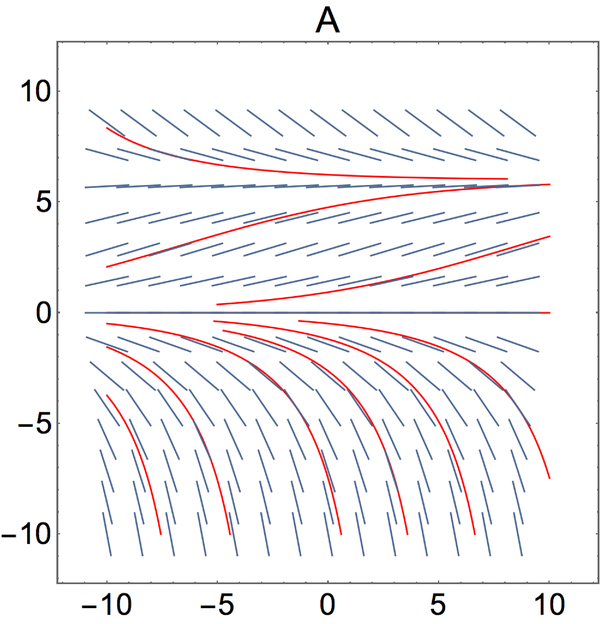
\includegraphics{direction_fields_A.png}
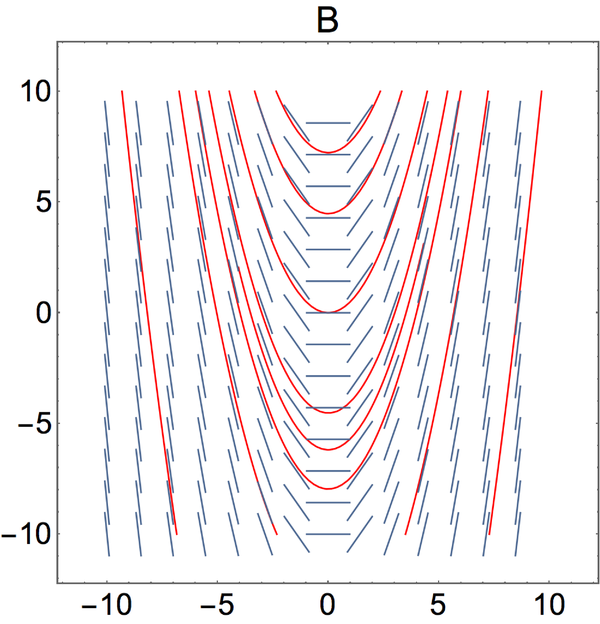
\includegraphics{direction_fields_B.png}
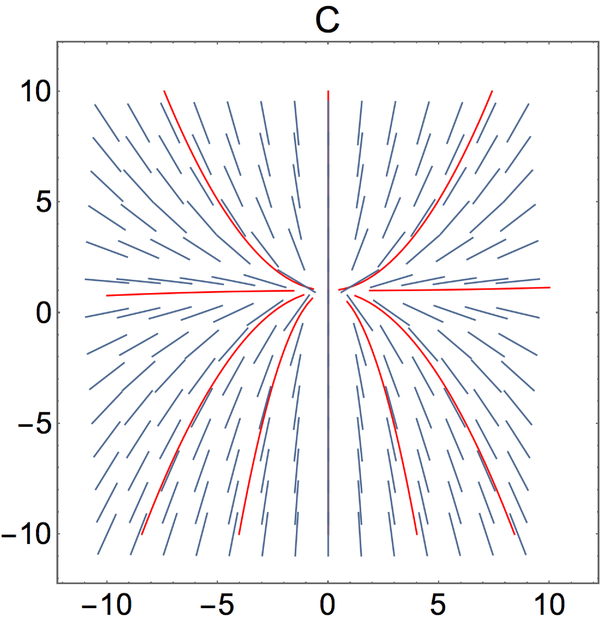
\includegraphics{direction_fields_C.png}

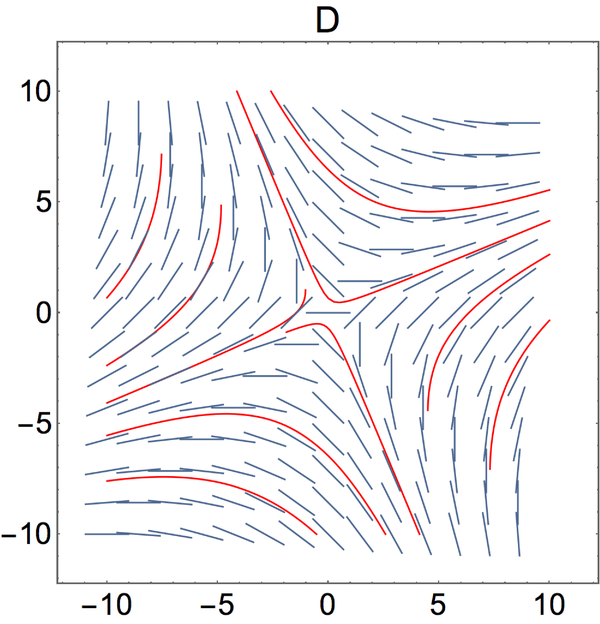
\includegraphics{direction_fields_D.png}
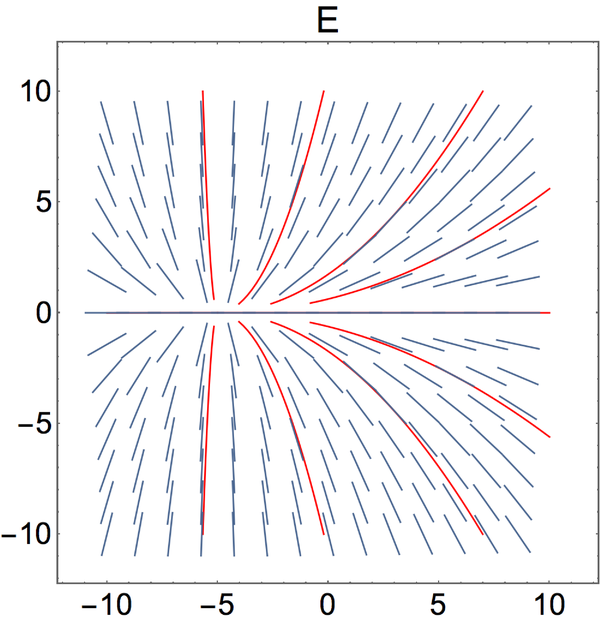
\includegraphics{direction_fields_E.png}
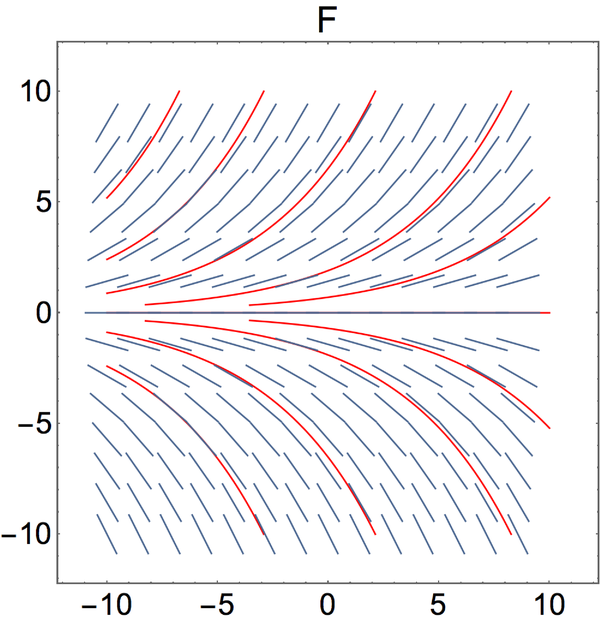
\includegraphics{direction_fields_F.png}

\subsection*{Solution}
\solstr{q}{e93bfe}



%%%%%%%%%%%%%%%%%%%%%%%%%%%%%%%%%
\newpage
%%%%%%%%%%%%%%%%%%%%%%%%%%%%%%%%%
\section{Separable equations I}
\label{sec:sepy}

\subsection*{Resources}
\begin{itemize}
    \item Video I: \url{https://www.khanacademy.org/math/differential-equations/first-order-differential-equations/separable-equations/v/separable-differential-equations-introduction} 
    \item Video II: \url{https://www.khanacademy.org/math/differential-equations/first-order-differential-equations/separable-equations/v/particular-solution-to-differential-equation-example}
    \item Text:\url{http://tutorial.math.lamar.edu/Classes/DE/Separable.aspx}
\end{itemize}

\subsection*{Comment}
Let's start with a fundamental equation:
\begin{equation}
    \frac{dy}{dt} = y
\end{equation}
This is saying that the slope (the rate of change of y) linearly depends on $y$. That is, that as the value of y increases, the slope also increases; a positive feedback loop. In fact, you get an exponentially-increasing function.

So one aim of this course is to be able to solve such equations mathematically. But I also want you to understand the ``physical'' meaning of the relation between $y$ and its slope, and how this leads to such a fundamental function such as an exponential.

\subsection*{Challenge}
Considering the equation
\begin{equation}
    \frac{dy}{dt} = y
\end{equation}
solve for $y$.

\subsection*{Solution}
To check your answer, solve for $y(5)$ given the initial condition $y(0) = 1$.

$y(5) = 148.413$




%%%%%%%%%%%%%%%%%%%%%%%%%%%%%%%%%
\newpage
%%%%%%%%%%%%%%%%%%%%%%%%%%%%%%%%%
\section{Separable equations II}

\subsection*{Resources}
\begin{itemize}
    \item Video I: \url{https://www.khanacademy.org/math/differential-equations/first-order-differential-equations/separable-equations/v/separable-differential-equations-introduction} 
    \item Video II: \url{https://www.khanacademy.org/math/differential-equations/first-order-differential-equations/separable-equations/v/particular-solution-to-differential-equation-example}
    \item Text:\url{http://tutorial.math.lamar.edu/Classes/DE/Separable.aspx}
\end{itemize}

\subsection*{Challenge}
a) Now consider what is meant, physically speaking, by the relation:
\begin{equation}
    \frac{dy}{dt} = -y
\end{equation}
Why does it tend to zero for increasing $t$?

b) Solve for $y$.

\subsection*{Solution}
a) Please compare your solution with your partner or discuss with the teacher.

b) To check your answer, solve for $y(5)$ given the initial condition $y(0) = 1$.

$y(5) = 0.00674$





%%%%%%%%%%%%%%%%%%%%%%%%%%%%%%%%%
\newpage
%%%%%%%%%%%%%%%%%%%%%%%%%%%%%%%%%
\section{Separable equations III}

\subsection*{Resources}
\begin{itemize}
    \item Video I: \url{https://www.khanacademy.org/math/differential-equations/first-order-differential-equations/separable-equations/v/separable-differential-equations-introduction} 
    \item Video II: \url{https://www.khanacademy.org/math/differential-equations/first-order-differential-equations/separable-equations/v/particular-solution-to-differential-equation-example}
    \item Text:\url{http://tutorial.math.lamar.edu/Classes/DE/Separable.aspx}
\end{itemize}

\subsection*{Challenge}
a) Now consider when the slope of $y$ not only depends on $y$ but also on $t$:
\begin{equation}
    \frac{dy}{dt} = ty
\end{equation}

b) or on a constant $a$:
\begin{equation}
    \frac{dy}{dt} = ay
\end{equation}

See how the feedback is greater or lesser, depending on the constant or variable placed in front of $y$?

\subsection*{Solution}
a) Solve for $y(5)$ under the initial condition $y(0)=1$

268,337

b) Solve for $y(5)$ under the initial condition $y(0)=1$ and with $a=2$

22,026.5




%%%%%%%%%%%%%%%%%%%%%%%%%%%%%%%%%
\newpage
%%%%%%%%%%%%%%%%%%%%%%%%%%%%%%%%%
\section{Separable equations IV}

\subsection*{Resources}
\begin{itemize}
    \item Video I: \url{https://www.khanacademy.org/math/differential-equations/first-order-differential-equations/separable-equations/v/separable-differential-equations-introduction} 
    \item Video II: \url{https://www.khanacademy.org/math/differential-equations/first-order-differential-equations/separable-equations/v/particular-solution-to-differential-equation-example}
    \item Text:\url{http://tutorial.math.lamar.edu/Classes/DE/Separable.aspx}
\end{itemize}

\subsection*{Challenge}
Determine $y(t)$ for
\begin{equation}
    \frac{dy}{dt} = e^{t}
\end{equation}

Again, think about what is happening here. Do you see the link with challenge \ref{sec:sepy}? There we wrote in terms of $y$. Here we write in terms of $e^{t}$. Do you see they're the same thing?

\subsection*{Solution}
To check your answer, solve for $y(3)$ given the initial condition $y(0) = 1$.

$y(3) = 20.09$




%%%%%%%%%%%%%%%%%%%%%%%%%%%%%%%%%
\newpage
%%%%%%%%%%%%%%%%%%%%%%%%%%%%%%%%%
\section{Rate of growth}

\subsection*{Resources}
\begin{itemize}
    \item Video: \url{https://www.khanacademy.org/math/differential-equations/first-order-differential-equations/logistic-differential-equation/v/modeling-population-with-differential-equations}
\end{itemize}

\subsection*{Comment}
One interesting application of 1st-order differential equations is that of population growth.

\subsection*{Challenge}
Assuming there is no-limit on growth, a given bacteria would be able to reproduce at such a rate that the amount of bacteria measured in mg increases by 20\% every 25 hours. Derive an expression for the rate of growth.

\subsection*{Solution}
To check your answer, calculate the rate of growth when there are 20 mg of bacteria.
\emph{To ensure accuracy, you will need to maintain a large degree of precision during your calculations.}

0.146 mg/hour




%%%%%%%%%%%%%%%%%%%%%%%%%%%%%%%%%
\newpage
%%%%%%%%%%%%%%%%%%%%%%%%%%%%%%%%%
\section{Logistic equation}

\subsection*{Resources}
\begin{itemize}
    \item Videos: The 4 remaining logistic differential equation videos starting at: \url{https://www.khanacademy.org/math/differential-equations/first-order-differential-equations/logistic-differential-equation/v/logistic-differential-equation-intuition}
\end{itemize}

\subsection*{Comment}
We considered exponential growth, but in real life there is often a limit to this. This is where the logistic equation is useful.

\subsection*{Challenge}
Assuming there is no-limit on growth, a given bacteria would be able to reproduce at such a rate that the amount of bacteria measured in mg increases by 20\% every 25 hours. However, due to environmental factors the limiting (maximum) amount of bacteria that can exist in the system at any one time is 400 mg. Assuming an initial amount of bacteria of 20 mg, how much time must one wait to reach 100 mg of bacteria?

\subsection*{Solution}
253 hours




%%%%%%%%%%%%%%%%%%%%%%%%%%%%%%%%%
\newpage
%%%%%%%%%%%%%%%%%%%%%%%%%%%%%%%%%
\section{Autonomous differential equations}

\subsection*{Resources}
\begin{itemize}
    \item Wikipedia: \url{https://en.wikipedia.org/wiki/Autonomous_system_(mathematics)}
\end{itemize}

\subsection*{Challenge}
The logistic equation is an example of an autonomous differential equation.
Add the points of the autonomous differential equations in the following list:

1 point: $y' = cos(y)-5$

2 points: $y' = cos(y)/x - 5$

4 points: $y' = cos(y)/x - 5/x$

8 points: $y^2 = y' y+5$

16 points: $x y' = 5 y$

32 points: $y' = 1$

\subsection*{Solution}
\solint{f}{1227c7}



%%%%%%%%%%%%%%%%%%%%%%%%%%%%%%%%%
\newpage
%%%%%%%%%%%%%%%%%%%%%%%%%%%%%%%%%
\section{The stability of solutions I}

\subsection*{Resources}
\begin{itemize}
    \item Text: \url{http://tutorial.math.lamar.edu/Classes/DE/EquilibriumSolutions.aspx}
    \item Text: \url{http://www.math.psu.edu/tseng/class/Math251/Notes-1st\%20order\%20ODE\%20pt2.pdf}
\end{itemize}

\subsection*{Challenge}
Considering the logistic equation $N'=0.2N(1-N/6)$, make 3 separate lists containing any equilibrium, semi-stable and unstable y-values.

To check your answer, sum the value of each list. If there are no values in a list, enter $-999$ to check the result.

\subsection*{Solution}
\subsubsection*{Stable}
\solint{g}{4a4314}

\subsubsection*{Semi-stable}
\solint{h}{9df203}

\subsubsection*{Unstable}
\solint{j}{17cb7f}




%%%%%%%%%%%%%%%%%%%%%%%%%%%%%%%%%
\newpage
%%%%%%%%%%%%%%%%%%%%%%%%%%%%%%%%%
\section{The stability of solutions II}

\subsection*{Resources}
\begin{itemize}
    \item Text: \url{http://tutorial.math.lamar.edu/Classes/DE/EquilibriumSolutions.aspx}
    \item Text: \url{http://www.math.psu.edu/tseng/class/Math251/Notes-1st\%20order\%20ODE\%20pt2.pdf}
\end{itemize}

\subsection*{Challenge}
Considering the differential equation $y'=(y^2-16)(y+3)^2$, make 3 separate lists containing any equilibrium, semi-stable and unstable y-values.

To check your answer, sum the value of each list. If there are no values in a list, simply enter ``none'' to check the result.

\subsection*{Solution}
\subsubsection*{Stable}
\solint{k}{ffc446}

\subsubsection*{Semi-stable}
\solint{z}{f76cc4}

\subsubsection*{Unstable}
\solint{x}{bf947d}



\iffalse
%\iffalse
%%%%%%%%%%%%%%%%%%%%%%%%%%%%%%%%%
\newpage
%%%%%%%%%%%%%%%%%%%%%%%%%%%%%%%%%
\section{Euler's method}

\subsection*{Resources}
\begin{itemize}
    \item Videos and exersizes in the ``Euler's Method'' section of Khan academy: \url{https://www.khanacademy.org/math/differential-equations/first-order-differential-equations/eulers-method-tutorial/v/eulers-method}
    \item Text: \url{http://tutorial.math.lamar.edu/Classes/DE/EulersMethod.aspx}
\end{itemize}

\subsection*{Challenge}
Considering the differential equation $y'=10-y$, an initial value of $y(0)=1$ and a step size of $\Delta x = 0.2$, use Euler's method to estimate the value of $y(x=1)$. The actual solution, $y(x)=10-9e^{-x}$, is shown below.

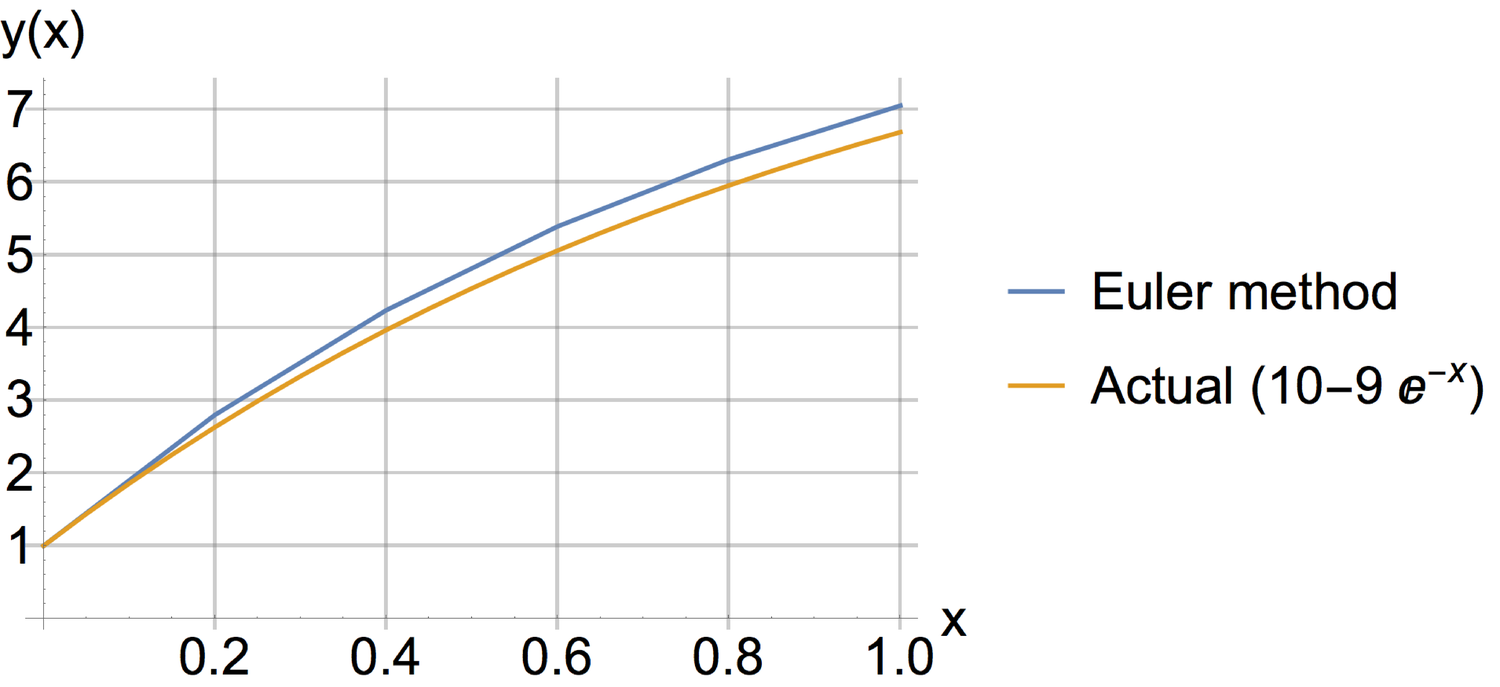
\includegraphics{eulers_method.png}

\subsection*{Solution}
\six{}

\hash{c}{1f90fa} 
% It would be nice to see if this error actually goes to zero in the end.




%%%%%%%%%%%%%%%%%%%%%%%%%%%%%%%%%
\newpage
%%%%%%%%%%%%%%%%%%%%%%%%%%%%%%%%%
\section{Exact differential equations: derivation}

\subsection*{Resources}
\begin{itemize}
    \item Videos: \url{https://www.khanacademy.org/math/differential-equations/first-order-differential-equations/exact-equations/v/exact-equations-intuition-1-proofy}
\end{itemize}

\subsection*{Challenge}
Please follow the two videos on derivation and intuition regarding exact differential equations starting at the video listed above.

If
\begin{equation}
    \frac{d \psi(x,y)}{dx} = 2xy + x^2y' - (x+y)/100
\end{equation}

what is $\displaystyle \frac{\partial \psi}{\partial x}$?

To check your answer, substitute $x=3.1$ and $y=-2$ into the resulting equation.

\subsection*{Solution}
\six{}

\hash{v}{f7f178}
% Note that video is not so clear about psi being a full rather than partial derivative. This question should help address this problem.




%%%%%%%%%%%%%%%%%%%%%%%%%%%%%%%%%
\newpage
%%%%%%%%%%%%%%%%%%%%%%%%%%%%%%%%%
\section{Exact differential equations: possible solutions given $\psi_x$}

\subsection*{Resources}
\begin{itemize}
    \item Videos: Exact equations intuition 1,2 and examples 1,2,3 starting from \url{https://www.khanacademy.org/math/differential-equations/first-order-differential-equations/exact-equations/v/exact-equations-intuition-1-proofy}
    \item Text: \url{http://tutorial.math.lamar.edu/Classes/DE/Exact.aspx}
\end{itemize}

\subsection*{Challenge}
Sum the points of all the possible solutions to the integral of the partial-differential equation:
\begin{equation}
    \psi_x = 6x - 3e^x sin(y)
\end{equation}

1 point: $\psi(x,y) = 3x^2-3e^x sin(y) + 4$

2 points: $\psi(x,y) = 3x^2-3e^x sin(y) + x$

4 points: $\psi(x,y) = 3x^2-3e^x sin(y) + y$

8 points: $\psi(x,y) = 3x^2-3e^x sin(y) + yx$

16 points: $\psi(x,y) = 3x^2-3e^x sin(y) + y^2$

32 points: $\psi(x,y) = 3x^2-3e^x sin(y) + 5 sin(y)$

64 points: $\psi(x,y) = 3x^2-3e^x sin(y) + 5 sin(y)cos(x)$

\subsection*{Solution}
\six{}

\hash{b}{408993} 




%%%%%%%%%%%%%%%%%%%%%%%%%%%%%%%%%
\newpage
%%%%%%%%%%%%%%%%%%%%%%%%%%%%%%%%%
\section{Exact differential equations: identification}
\label{sec:edeid}

\subsection*{Resources}
\begin{itemize}
    \item Videos: Exact equations intuition 1,2 starting from \url{https://www.khanacademy.org/math/differential-equations/first-order-differential-equations/exact-equations/v/exact-equations-intuition-1-proofy}
    \item Text: \url{http://tutorial.math.lamar.edu/Classes/DE/Exact.aspx}
\end{itemize}

\subsection*{Challenge}
Sum the points of the equations below that are exact differential equations:

1 point: $\displaystyle (3x^2y+8xy^2) dx + (x^3 + 8x^2y + 12 y^2) dy = 0$ % A

2 points: $\displaystyle sin(x) cos(y) dx + cos(x) sin(y) dy = 0$ % B

4 points: $\displaystyle sin(x) cos(y) dx + sin(x) sin(y) dy = 0$ % C

8 points: $\displaystyle \frac{dx}{x} + \frac{dy}{y} = 0$ % D

16 points: $\displaystyle -\frac{y dx + x dy}{x^2} = 0 $ % E

32 points: $\displaystyle -\frac{y dx - x dy}{x^2} = 0$ % F


\subsection*{Solution}
\six{}

\hash{n}{868f48} 




%%%%%%%%%%%%%%%%%%%%%%%%%%%%%%%%%
\newpage
%%%%%%%%%%%%%%%%%%%%%%%%%%%%%%%%%
\section{Exact differential equations: solving}

\subsection*{Resources}
\begin{itemize}
    \item Videos: Exact equations examples 1,2,3 starting from \url{https://www.khanacademy.org/math/differential-equations/first-order-differential-equations/exact-equations/v/exact-equations-example-1}
    \item Text: \url{http://tutorial.math.lamar.edu/Classes/DE/Exact.aspx}
\end{itemize}

\subsection*{Challenge}
In challenge \ref{sec:edeid} you should have identified 4 exact differential equations. Considering each of the 4 EDE's in order, try to solve the EDE's applying the following conditions:

\subsubsection{1st EDE}
Do not try to solve this one.

\subsubsection{2nd EDE}
Use the condition $y(\pi/4)=\pi/4$ to find an explicit solution for the equation and then evaluate $y$ at $x=\pi$.

\subsubsection{3rd EDE}
Use the condition $y(1)=3$ to find an explicit solution for the equation and then evaluate $y$ at $x=4$.

\subsubsection{4th EDE}
Use the condition $y(1)=2$ to find an explicit solution for the equation and then evaluate $y$ at $x=1$.


\subsection*{Solution}

\subsubsection{2nd EDE}
\six{}

\hash{m}{af87e2}

\subsubsection{3rd EDE}
\six{}

\hash{aa}{d01c3d}

\subsubsection{4th EDE}
\six{}

\hash{bb}{5e1074}




%%%%%%%%%%%%%%%%%%%%%%%%%%%%%%%%%
\newpage
%%%%%%%%%%%%%%%%%%%%%%%%%%%%%%%%%
\section{Exact differential equations: a useful integration method}

\subsection*{Challenge}
Obtain an expression for $g(x)$ in terms of $f(x)$ in the following integral:

\begin{equation}
    \int \frac{f'(x)}{f(x)} dx = g(x)
\end{equation}

ie, you should be able to re-write $g(x)$ in terms of a simple (non-integral) function of $f(x)$, in the form $g(x) = \cdots$.

\subsection*{Solution}
You can check your answer by putting a function of $x$ into $f(x)$.




%%%%%%%%%%%%%%%%%%%%%%%%%%%%%%%%%
\newpage
%%%%%%%%%%%%%%%%%%%%%%%%%%%%%%%%%
\section{Exact differential equations: integrating factors}
\label{sec:edeif}

\subsection*{Resources}
\begin{itemize}
    \item Videos: Integrating factors 1,2 starting from \url{https://www.khanacademy.org/math/differential-equations/first-order-differential-equations/exact-equations/v/integrating-factors-1}
\end{itemize}

\section*{Comment}
Note that in the videos, Sal Khan does an example considering an integrating factor of $\mu(x)$, but in some cases $\mu(y)$ leads to a solution more easily. You may need to try both to determine an answer.

\subsection*{Challenge}
Solve the exact differential equations below using integrating factors.

1. Solve the equation below using an integrating factor. Place the solution in the form $f(x,y) = C$, then calculate the value of $C$ when substituting $x=2$ and $y=1$ into the equation. Do not try to solve the equation to get it in the form $y(x)=\cdots$.

\begin{equation}
    \label{eq:edeif1}
    y dx + (2 x y - e^{-2 y}) dy = 0
\end{equation}

2. Calculate the integrating factor for the following equation. To check your answer, substitute $x=1$ or $y=1$ into any final expression, assuming an integration constant of zero.

\begin{equation}
    \label{eq:edeif2}
    y(3x-y) dx + x(x-y)dy = 0
\end{equation}

3. Show that $1/(x^y+y^2)$ is an integrating factor for the equation
\begin{equation}
    x dx + y dy + 4 y^3 (x^2 + y^2)dy = 0
\end{equation}

\subsection*{Solution}
Challenge related to equation \ref{eq:edeif1}: \hash{cc}{bb15d6}

Challenge related to equation \ref{eq:edeif2}: \hash{dd}{6a8742}




%%%%%%%%%%%%%%%%%%%%%%%%%%%%%%%%%
\newpage
%%%%%%%%%%%%%%%%%%%%%%%%%%%%%%%%%
\section{Exact differential equations: integrating factor derivation}
\label{sec:intfacderiv}

\subsection*{Challenge}
1. Starting from the equation

\begin{equation}
    \mu(x,y) M(x,y) dx + \mu(x,y) N(x,y) dy = 0
\end{equation}

show that if the integrating factor $\mu$ is only a function of $x$, then

\begin{equation}
    \label{eq:intfacmux}
    \mu_x = \mu \left ( \frac{M_y-N_x}{N} \right )
\end{equation}

2. Do the same, assuming that $\mu$ is only a function of $y$.

% NT do something for linear equations mu=e^\int(a)




%%%%%%%%%%%%%%%%%%%%%%%%%%%%%%%%%
\newpage
%%%%%%%%%%%%%%%%%%%%%%%%%%%%%%%%%
\section{Exact differential equations: integrating factor calculation}
\label{sec:edeifcalc}

\section*{Comment}
Without proof, we can use equation \ref{eq:intfacmux} to gain information about the existance of an integration factor. If $\left ( \frac{M_y-N_x}{N} \right )$ is a function of $x$ only, then we know that the integration factor is only a function of $x$, and it can be solved for by integration of equation \ref{eq:intfacmux}. The same can be said for $\mu(y)$ that you derived an expression for in challenge \ref{sec:intfacderiv}.

\subsection*{Challenge}
Use equations from section \ref{sec:intfacderiv} and information provided in the comment here to determine the integrating factor for

\begin{equation}
    \label{eq:edeifcalc1}
    e^x dx + (e^x Cot(y) + 2y Csc(y)) dy = 0
\end{equation}

and

\begin{equation}
    \label{eq:edeifcalc2}
    (x-y^2) dx + 2xy dy = 0
\end{equation}

To check your answer, for both cases substitute $x=\pi$ or $y=\pi$ into the integrating factor, and assume an integration constant of 1.

\subsection*{Solution}


Equation \ref{eq:edeifcalc1}: \hash{ee}{51a0ae}

Equation \ref{eq:edeifcalc2}: \hash{ff}{a56bce}




%%%%%%%%%%%%%%%%%%%%%%%%%%%%%%%%%
\newpage
%%%%%%%%%%%%%%%%%%%%%%%%%%%%%%%%%
\section{Summary of 1st-order differential equations}

\subsection*{Challenge}
1. Create a flowchart describing how you will approach solving a general 1st-order differential equation.

% Linear, Separable, Exact (with and without integration factors)
2. Solve the following 1st-order differential equations:

\begin{equation}
    \label{eq:1odegen1}
    y' - 4y = 8x + 3
\end{equation}
evaluated at $x=1$.

\begin{equation}
    \label{eq:1odegen2}
    4yy' = 8x + 3
\end{equation}
assuming an integration constant of zero and evaluating the final equation at $x=2$.

\begin{equation}
    \label{eq:1odegen3}
    y' + 4y = e^{-8x}
\end{equation}
assuming an integration constant of zero and evaluating the final equation at $x=1/8$.

\subsection*{Solution}
Equation \ref{eq:1odegen1}: \hash{qq}{a43ab2}

Equation \ref{eq:1odegen2}: \hash{rr}{990bfa}

Equation \ref{eq:1odegen3}: \hash{ss}{91989d}

\fi


% Benouli and substitution

% More advanced topics are in Paul's notes, but first check how much time is remaining.

% Do I need to add more challenges for simple 1st order linear equations?

\chapter{2nd-order differential equations}
\section{Hooke's law}

\subsection*{Resources}

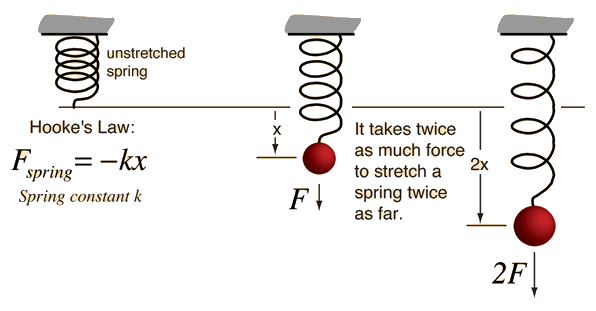
\includegraphics[scale=0.5]{hook.png}\\
\emph{(\href{http://hyperphysics.phy-astr.gsu.edu/hbase/imgmec/hook.gif}{Image} from HyperPhysics by Rod Nave, Georgia State University)}

\subsection*{Challenge}
2nd-order differential equations deal with oscillations.

Considering Hooke's law, what are $A$ and $C$ in the following equation?
\begin{equation}
    A x'' + C x = 0
\end{equation}

To check your answer, substitute a mass of \SI{2}{kg} and spring-constant of \SI{3}{kg/s^2} as appropriate.

\subsection*{Solution}
Enter only numberical values without units such as kg.

A: \hash{gg}{4e5fe6}

C: \hash{hh}{6a7015}




%%%%%%%%%%%%%%%%%%%%%%%%%%%%%%%%%
\newpage
%%%%%%%%%%%%%%%%%%%%%%%%%%%%%%%%%
\section{Exponentials and trigonometry}

\subsection*{Resources}
\begin{itemize}
    \item Text: \url{https://www.phy.duke.edu/~rgb/Class/phy51/phy51/node15.html}
\end{itemize}

\subsection*{Challenge}
Write $sin(x)$ and $cos(x)$ in exponential form.

\subsection*{Solution}

Check your answer with someone if you are unsure.


\timebox




%%%%%%%%%%%%%%%%%%%%%%%%%%%%%%%%%
\newpage
%%%%%%%%%%%%%%%%%%%%%%%%%%%%%%%%%
\section{Characteristic equation: understanding}

\subsection*{Resources}
\begin{itemize}
    \item Text: \url{http://tutorial.math.lamar.edu/getfile.aspx?file=S,88,N}
\end{itemize}

\subsection*{Comment}
A homogeneous (ie, equal to zero) second-order differential equation typically takes the form:

\begin{equation}
    A \frac{d^2y}{dt^2} + B \frac{dy}{dt} + C y = 0
\end{equation}

The first (A) term describes acceleration, while the third (C) term is the force-constant term (something like the ``stiffness'' of the spring). The second (B) term could describe a frictional force that is proportional to the velocity ($dy/dt$). Due to its relation with oscillation (and by extension, sines and cosines which can be expressed in terms of exponentials) we can typically assume an exponential-form solution to the differential equation.

\subsection*{Challenge}
Show that, assuming that all solutions to a 2nd-order differential equation of the form above will have solutions $y(t)=e^{rt}$, the value of $r$ can in principle be determined by solving the following a quadratic equation of the form
\begin{equation}
    A r^2 + Br + C = 0
\end{equation}

\subsection*{Solution}
If you are unsure of your derivation, please ask someone.

\timebox




%%%%%%%%%%%%%%%%%%%%%%%%%%%%%%%%%
\newpage
%%%%%%%%%%%%%%%%%%%%%%%%%%%%%%%%%
\section{Characteristic equation: roots}

\subsection*{Resources}
\begin{itemize}
    \item Text: \url{http://tutorial.math.lamar.edu/getfile.aspx?file=S,88,N}
\end{itemize}

\subsection*{Challenge}
Sum the points of the differential equations that have characteristic equations with
\begin{itemize}
    \item Real, distinct roots
    \item Complex roots
    \item Equal roots
\end{itemize}

1 point: $\displaystyle -3 y'' - 5 y' + 2 y = 0$ % C

2 points: $\displaystyle 3 y'' - 4 y' + 3 y = 0$ % E

4 points: $\displaystyle 3 y'' - 6 y' + 3 y = 0$ % B

8 points: $\displaystyle 3 y'' - 5 y' + 2 y = 0$ % F

16 points: $\displaystyle 3 y'' - 5 y' + 4 y = 0$ % D

32 points: $\displaystyle 3 y'' + 5 y' + 2 y = 0$ % A

\subsection*{Solution}

\begin{itemize}
    \item Real, distinct roots: \hash{ii}{064a6e}
    \item Complex roots: \hash{jj}{50385e}
    \item Equal roots: \hash{kk}{70cd8f}
\end{itemize}

\timebox




%%%%%%%%%%%%%%%%%%%%%%%%%%%%%%%%%
\newpage
%%%%%%%%%%%%%%%%%%%%%%%%%%%%%%%%%
\section{Characteristic equation: real roots with positive B}

\subsection*{Resources}
\begin{itemize}
    \item Text: \url{http://tutorial.math.lamar.edu/getfile.aspx?file=S,94,N}
\end{itemize}

\subsection*{Comment}

\subsection*{Challenge}
Solve the following 2nd-order differential equation that has real roots:

\begin{equation}
    \label{eq:ccrrpb}
    y'' + 3 y' + 2 y = 0
\end{equation}

with initial conditions $y(0)=5$ and $y'(0)=-8$.

To check your answer, substitute $t=1$ into the final expression.


\subsection*{Solution}
\hash{mm}{9b9be5}




%%%%%%%%%%%%%%%%%%%%%%%%%%%%%%%%%
\newpage
%%%%%%%%%%%%%%%%%%%%%%%%%%%%%%%%%
\section{Characteristic equation: real roots with negative B}

\subsection*{Resources}
\begin{itemize}
    \item Text: \url{http://tutorial.math.lamar.edu/getfile.aspx?file=S,94,N}
\end{itemize}

\subsection*{Challenge}
Solve the following 2nd-order differential equation that has real roots. 

\begin{equation}
    y'' - 3 y' + 2 y = 0
\end{equation}

with initial conditions $y(0)=5$ and $y'(0)=8$. Substitue $t=1$ into the final expression to check your answer.

Note that this equation is the same as equation \ref{eq:ccrrpb}, but simply the dampening (friction) term B has been changed from positive to negative.


\subsection*{Solution}
\hash{nn}{473835}

\timebox




%%%%%%%%%%%%%%%%%%%%%%%%%%%%%%%%%
\newpage
%%%%%%%%%%%%%%%%%%%%%%%%%%%%%%%%%
\section{Characteristic equation: B in equations with real roots}

\subsection*{Challenge}

\emph{(Note that there are two parts to this challenge.)}

1. Considering real root, sum the points of the following true statements:

Considering the equation

\begin{equation}
    A y'' + B y' + C y = 0
\end{equation}

1 point: Positive damping (positive B) leads to solutions with exponentials with positive exponents.

2 points: Positive damping (positive B) leads to solutions with exponentials with negative exponents.

4 points: Negative damping (negative B) leads to solutions with exponentials with positive exponents.

8 points: Negative damping (negative B) leads to solutions with exponentials with negative exponents.

16 points: Exponentials with positive exponents (eg, $e^{t}$) lead to exponential growth (instability).

32 points: Exponentials with negative exponents (eg, $e^{-t}$) lead to exponential growth (instability).

64 points: Exponentials with positive exponents (eg, $e^{t}$) lead to a damped signal (stability).

128 points: Exponentials with negative exponents (eg, $e^{-t}$) lead to damped signal (stability).

\vspace{2em}

2. Write a sentence summarising your understanding of the significance of having a positive or negative coefficient of $B$ when the roots are real.


\subsection*{Solution}
\hash{oo}{fa6adf}

\timebox




%%%%%%%%%%%%%%%%%%%%%%%%%%%%%%%%%
\newpage
%%%%%%%%%%%%%%%%%%%%%%%%%%%%%%%%%
\section{Characteristic equation: equal roots}

\subsection*{Resources}
\begin{itemize}
    \item Text: \url{http://tutorial.math.lamar.edu/getfile.aspx?file=S,96,N}
\end{itemize}

\subsection*{Comment}
It is not necessary to follow the full derivation in the suggested resource.

\subsection*{Challenge}
Solve the equation
\begin{equation}
    y'' - 2y' + y = 0
\end{equation}

To check your solution, substitute $t=1$ into the equation and assume $c_1 = c_2 = 1$.

\subsection*{Solution}
\hash{pp}{ff7ca2}

\timebox




%%%%%%%%%%%%%%%%%%%%%%%%%%%%%%%%%
\newpage
%%%%%%%%%%%%%%%%%%%%%%%%%%%%%%%%%
\section{Characteristic equation: complex roots with B=0}

\subsection*{Resources}
\begin{itemize}
    \item Text: \url{http://tutorial.math.lamar.edu/getfile.aspx?file=S,96,N}
\end{itemize}

\subsection*{Challenge}
1. Assuming there is no damping term (ie, $B=0$) show that the roots for the differential equation
\begin{equation}
    A y'' + Cy = 0
\end{equation}
are $\pm i \sqrt{C/A}$.

2. Solve the following ODE:
\begin{equation}
    \label{eq:cecr}
    y'' + 4 \pi^2 y = 0
\end{equation}

To check your answer, assume integration constants of 1 and calculate $y(\pi/2)$.

\subsection*{Solution}
Solution to part 2: \hash{qq}{7eb2c9}

\timebox




%%%%%%%%%%%%%%%%%%%%%%%%%%%%%%%%%
\newpage
%%%%%%%%%%%%%%%%%%%%%%%%%%%%%%%%%
\section{Characteristic equation: complex roots with positive B}

\subsection*{Resources}
\begin{itemize}
    \item Text: \url{http://tutorial.math.lamar.edu/getfile.aspx?file=S,96,N}
\end{itemize}

\subsection*{Challenge}
Solve the following ODE:
\begin{equation}
    y'' + y' + y = 0
\end{equation}

To check your answer, assume integration constants of 1 and calculate $y(\pi/2)$.

\subsection*{Solution}
\hash{rr}{1d0cb5}

\timebox




%%%%%%%%%%%%%%%%%%%%%%%%%%%%%%%%%
\newpage
%%%%%%%%%%%%%%%%%%%%%%%%%%%%%%%%%
\section{Characteristic equation: complex roots with negative B}

\subsection*{Resources}
\begin{itemize}
    \item Text: \url{http://tutorial.math.lamar.edu/getfile.aspx?file=S,96,N}
\end{itemize}

\subsection*{Challenge}
Solve the following ODE:
\begin{equation}
    y'' - y' + y = 0
\end{equation}

To check your answer, assume integration constants of 1 and calculate $y(\pi/2)$.

\subsection*{Solution}
\hash{ss}{caf35b}

\timebox




%%%%%%%%%%%%%%%%%%%%%%%%%%%%%%%%%
\newpage
%%%%%%%%%%%%%%%%%%%%%%%%%%%%%%%%%
\section{Damping}
\label{sec:damping}

\subsection*{Resources}
\begin{itemize}
    \item Wikipedia: https://en.wikipedia.org/wiki/Damping
\end{itemize}

\subsection*{Challenge}
Of the 6 functions shown in the graph, place the 3 that correspond to overdamped, critially damped and underdamped in the order mentioned in this sentence.

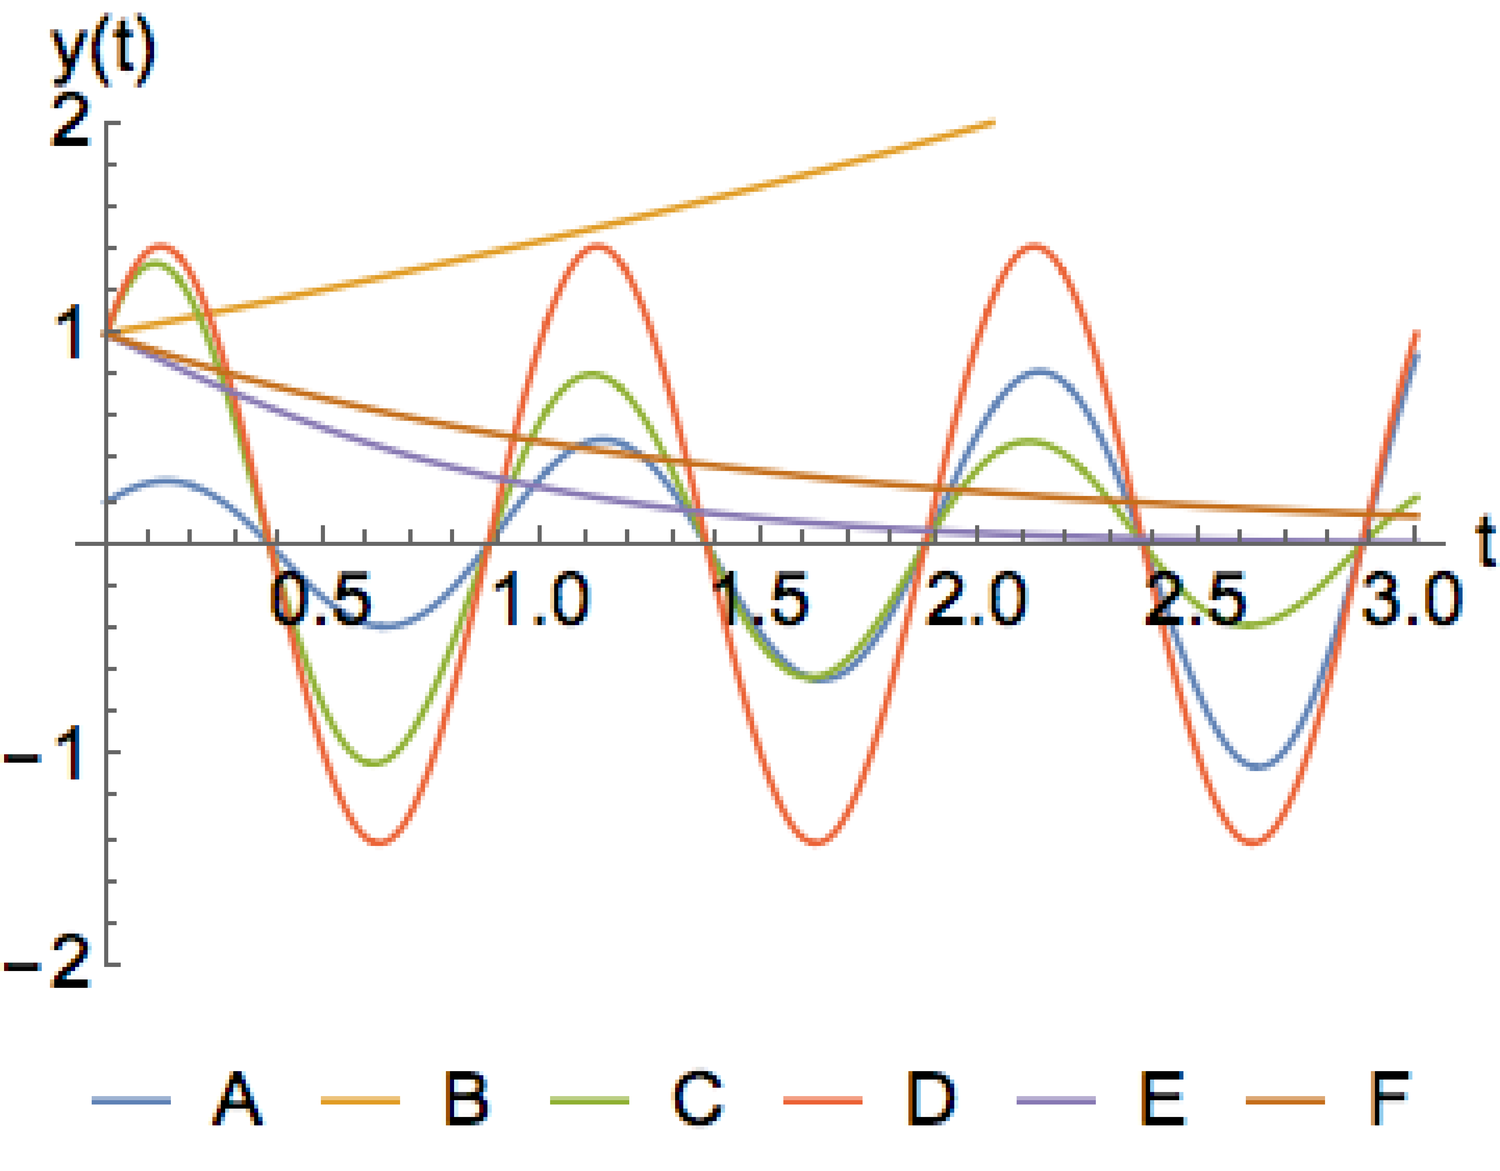
\includegraphics{damping.png}

\subsection*{Solution}
(eg, ``abc'')

\hash{tt}{060b2a}

\timebox



%%%%%%%%%%%%%%%%%%%%%%%%%%%%%%%%%
\newpage
%%%%%%%%%%%%%%%%%%%%%%%%%%%%%%%%%
\section{Damping and 2nd-order differential equations}

\subsection*{Challenge}
1. The 6 functions shown in the graph in challenge \ref{sec:damping} may represent solutions of a 2nd-order differential equation. Place the solutions A-F in the order shown below. Note that one of the descriptions below is impossible, and you should ignore that one.

I. Solution of a 2nd-order differential equation with real roots and positive B.

II. Solution of a 2nd-order differential equation with real roots and negative B.

III. Solution of a 2nd-order differential equation with real roots and B=0.

IV. Solution of a 2nd-order differential equation with equal roots.

V. Solution of a 2nd-order differential equation with complex roots and B=0.

VI. Solution of a 2nd-order differential equation with complex roots and positive B.

VII. Solution of a 2nd-order differential equation with complex roots and negative B.

\vspace{1em}
2. Write one sentence stating why one of the above solutions is impossible.

\subsection*{Solution}
(eg, ``abcdef'')

\hash{uu}{a96870}

\timebox



% One problem proving that one case is a fundamental solution
%%%%%%%%%%%%%%%%%%%%%%%%%%%%%%%%%%
%\newpage
%%%%%%%%%%%%%%%%%%%%%%%%%%%%%%%%%%
%\section{The Wronskian}
%
%\subsection*{Resources}
%\begin{itemize}
%    \item 
%\end{itemize}
%
%\subsection*{Challenge}
%Imagine you need to write a letter to a student, explaining what the Wronskian is, where it comes from, and how it is useful in determining the validity of fundamental sets of solutions. You may assume the student knows the formulas for solving different forms (complex, real and equal-roots) of 2nd-order ODE's with the characteristic equation method, but does not know what is meant by a ``fundamental solution'', doesn't understand why such fundamental solutions are sums of two terms, and does not know about the Wronskian. You may use the suggested resource to help formulate your letter. The student also would like to know about the connection of the Wronskian to linear independence and how this is related to the fundamental solutions (ie, why it matters that the two terms of the fundamental solutions are linearly independent).
%
%\emph{Suggested length: 1 A4 sheet.}
%
%\subsection*{Solution}
%Please give the letter to the teacher for posting. The teacher will check the depth of your understanding prior to posting.
%
%\timebox




%%%%%%%%%%%%%%%%%%%%%%%%%%%%%%%%%
%\newpage
%%%%%%%%%%%%%%%%%%%%%%%%%%%%%%%%%
%\section{Characteristic equation: exersizes}

%\subsection*{Challenge}
%Solve the following 2nd-order differential equations:

%\begin{equation}
    
%\end{equation}

%\subsection*{Solution}
%(eg, ``abcdef'')

%\hash{uu}{a96870}

%\timebox

%\chapter{Characteristics of solutions}
%\section{Free vibration of a spring (review)}

\subsection*{Challenge}
Consider a mass on a spring undergoing vibration with no damping or external forcing, just as you considered in challenge \ref{sec:hooke}.

Show that the position of the mass as a function of time can be given by
\begin{equation}
    \label{eq:freevib}
    x(t) = C_1 \sin \omega_0 t + C_2 \cos \omega_0 t
\end{equation}
where $C_1$ and $C_2$ are constants. 

\subsection*{Solution}
Please discuss with the teacher or your peers if you have any difficulty.




%%%%%%%%%%%%%%%%%%%%%%%%%%%%%%%%
\newpage
%%%%%%%%%%%%%%%%%%%%%%%%%%%%%%%%
\section{Phase-shift}

\subsection*{Comment}
Using the trigonometric identity
\begin{equation}
    \cos(\alpha \pm \beta) = \cos \alpha \cos \beta \mp \sin \alpha \sin \beta
\end{equation}
it is possible to write equation \ref{eq:freevib} as
\begin{equation}
    x(t) = C_3 \cos(\omega_0 t - \phi)
\end{equation}
where $C_1 = C_3 \cos \phi$ and $C_2 = C_3 \sin \phi$, while the magnitude of $C_3$ can be found using $C_3^2 = C_1^2 + C_2^2$.

\subsection*{Challenge}
Re-writing sine as a phase-shifted cosine; ie, $\sin \omega_0 t$ becoming $\cos (\omega_0 t - \phi)$; if $\omega_0 = 1$, what is $\phi$ (use the lowest-possible positive solution)?

\subsection*{Solution}
\soltwodp{f}{f97726}




%%%%%%%%%%%%%%%%%%%%%%%%%%%%%%%%
\newpage
%%%%%%%%%%%%%%%%%%%%%%%%%%%%%%%%
\section{Derivation of a periodically-forced system}

\subsection*{Challenge}
Now consider that there is some external forcing of the form $F \cos \omega t$ where $F$ is some constant.
Note that $\omega$ is the frequency at which the forcing varies, and $\omega_0^2 = k/m$ is the ``natural frequency'' of the unforced system.

Assuming $\omega \ne \omega_0$, show that the position of the forced system as a function of time can be given by
\begin{equation}
    \label{eq:forcedpostime}
    x(t) = C_3 \cos(\omega_0 t - \phi) + \frac{F}{m(\omega_0^2 - \omega^2)} \cos \omega t
\end{equation}




%%%%%%%%%%%%%%%%%%%%%%%%%%%%%%%%
\newpage
%%%%%%%%%%%%%%%%%%%%%%%%%%%%%%%%
\section{Beating equation}

\subsection*{Challenge}
\emph{Assuming that the mass on the spring starts at rest at position ``0''}, solve for the constant $C_3$ and the phase-shift $\phi$, then use trigonometric identity
\begin{equation}
    \cos \alpha - \cos \beta = 2 \sin \left( \frac{\alpha - \beta}{2} t \right) \sin \left( \frac{\alpha + \beta}{2} t \right)
\end{equation}
to show that the position of the mass as described in equation \ref{eq:forcedpostime} can be given by
\begin{equation}
    x(t) = \frac{2 F}{m(\omega_0^2 - \omega^2)} \sin \left( \frac{\omega - \omega_0}{2} t \right) \sin \left( \frac{\omega + \omega_0}{2} t \right)
\end{equation}




%%%%%%%%%%%%%%%%%%%%%%%%%%%%%%%%
\newpage
%%%%%%%%%%%%%%%%%%%%%%%%%%%%%%%%
\section{Beating explanation}

\section*{Resources}
\begin{itemize}
    \item \url{https://www.johndcook.com/blog/2013/02/22/undamped-forced-vibrations/}
    \item Video: \url{https://www.youtube.com/watch?v=v3ImPthjI3o}
\end{itemize}

\subsection*{Comment}
The equation that you obtained in the previous challenge demonstrates nicely the phenomenon of beating. You have a high-frequency wave multiplied by a low frequency wave. The image in the above resource depicts this visually very nicely and you can also hear a representation of this in sound with the video resource above.

\subsection*{Challenge}
Draw a graph depicting what happens as time evolves, and briefly explain what ``beating'' is and how it arises.




%%%%%%%%%%%%%%%%%%%%%%%%%%%%%%%%
\newpage
%%%%%%%%%%%%%%%%%%%%%%%%%%%%%%%%
\section{Resonance}

\section*{Resources}
\begin{itemize}
    \item \url{https://www.johndcook.com/blog/2013/02/22/undamped-forced-vibrations/}
    \item Video: \url{https://www.youtube.com/watch?v=v3ImPthjI3o}
\end{itemize}

\subsection*{Challenge}
Resonance occurs when the system is forced at its natural frequency (ie, $\omega = \omega_0$).

1. Show that when starting from position ``0'' at rest, when the system is driven at its natural frequency it evolves with time according to the equation
\begin{equation}
    x(t) = \frac{F}{2 m \omega_0} t \sin \omega t
\end{equation}

2. Draw a graph depicting what is happening as time evolves, and briefly explain what resonance is.

%\chapter{Laplace transformation}
%\section{Your first Laplace Transform calculations}

\subsection*{Resources}
\begin{itemize}
    \item Videos: The \textbf{four} Khan-academy videos starting at \url{https://www.khanacademy.org/math/differential-equations/laplace-transform/laplace-transform-tutorial/v/laplace-transform-1} % 8m+7:30+10+9 = 35:30
\end{itemize}

\subsection*{Comment}
The Laplace Transform is a powerful technique that has many uses beyond solving ODE's. It can however appear a bit abstract at first. Becoming comfortable with controlling and manipulating the transform will help provide confidence when using it to solve ODE's. The four videos in the resources above provide an excellent starting point for getting you comfortable with this powerful technique.

\subsection*{Challenge}
1. Calculate $\lap{1}$

2. Calculate $\lap{at}$

3. Calculate $\lap{Cos(at)}$

\subsection*{Solution}
To check your answer, substitute $s=1$ and $a=2$ into your final solution.

1. 1

2. 2

3. $\frac{1}{5}$




%%%%%%%%%%%%%%%%%%%%%%%%%%%%%%%%
\newpage
%%%%%%%%%%%%%%%%%%%%%%%%%%%%%%%%
\section{Laplace transform of a 3rd derivative}

\subsection*{Resources}
\begin{itemize} % Total video time: 20m
    \item Video I: \url{https://www.khanacademy.org/math/differential-equations/laplace-transform/properties-of-laplace-transform/v/laplace-transform-5} % 11:30
    \item Video II: \url{https://www.khanacademy.org/math/differential-equations/laplace-transform/properties-of-laplace-transform/v/laplace-transform-6} % 9:30
\end{itemize}

\subsection*{Challenge}
1. Calculate $\displaystyle \frac{d^3}{dt^3} \left( t e^{a t} \right)$

2. Given
\begin{equation}
    \lap{t e^{a t}} = \frac{1}{(a-s)^2}
\end{equation}
determine $\lap{3a^2 e^{at} + a^3te^{at}}$

\subsection*{Solution}
To check your answer, substitute $s=1$ and $a=2$ into your final solution.

-4




%%%%%%%%%%%%%%%%%%%%%%%%%%%%%%%%
\newpage
%%%%%%%%%%%%%%%%%%%%%%%%%%%%%%%%
\section{Shifting a transform}

\subsection*{Resources}
\begin{itemize}
    \item Video: \url{https://www.khanacademy.org/math/differential-equations/laplace-transform/properties-of-laplace-transform/v/more-laplace-transform-tools} %11m
\end{itemize}

\subsection*{Challenge}
Given
\begin{equation}
    \lap{Cosh(at)} = \frac{s}{s^2-a^2}
\end{equation}

1. What is $\lap{e^{3t} Cosh(5t)}$?

2. What is $f(t)$ in the equation $\lap{f(t)} = \frac{s-4}{(s-4)^2-100}$?

\subsection*{Solution}
To check your answer, substitute $s=2$ and $t=2$ as appropriate:

1. $0.0417$

2. $7.23 \times 10^{11}$




%%%%%%%%%%%%%%%%%%%%%%%%%%%%%%%%
\newpage
%%%%%%%%%%%%%%%%%%%%%%%%%%%%%%%%
\section{L'H\^opital's rule}

\subsection*{Resources}
\begin{itemize}
    \item Wikipedia: \url{https://en.wikipedia.org/wiki/L\%27H\%C3\%B4pital\%27s_rule}
\end{itemize}

\subsection*{Challenge}
1. Use L'H\^opital's rule to determine the limit of
\begin{equation}
    t e^{-st}
\end{equation}
as $x \rightarrow 0$.

2. Considering the case of
\begin{equation}
    \frac{t^n}{e^{st}}
\end{equation}
if we differentiate $n$ times with respect to $t$, what is the power of $t$ in the numerator? Note that $e^{st}$ is always constant, so by repeated differentiation we can apply L'H\^opital's rule even for $t^n$.

\subsection*{Solution}
1. \hash{ww}{76c8d4}

2. \hash{xx}{1592d7}




%%%%%%%%%%%%%%%%%%%%%%%%%%%%%%%%
\newpage
%%%%%%%%%%%%%%%%%%%%%%%%%%%%%%%%
\section{Laplace Transformation of the unit step function}

\subsection*{Resources}
\begin{itemize}
    \item Video: \url{https://www.khanacademy.org/math/differential-equations/laplace-transform/properties-of-laplace-transform/v/laplace-transform-of-the-unit-step-function} % 24m
\end{itemize}

\subsection*{Challenge}
Considering $U_c$ as the unit step-function at $c$, calculate the following Laplace transformations:

1. $\displaystyle \lap{U_0}$

2. $\displaystyle \lap{U_c}$

3. A 1-second pulse function starting at time $t=1$ with value $f(y)=1$ as shown in the graph below:
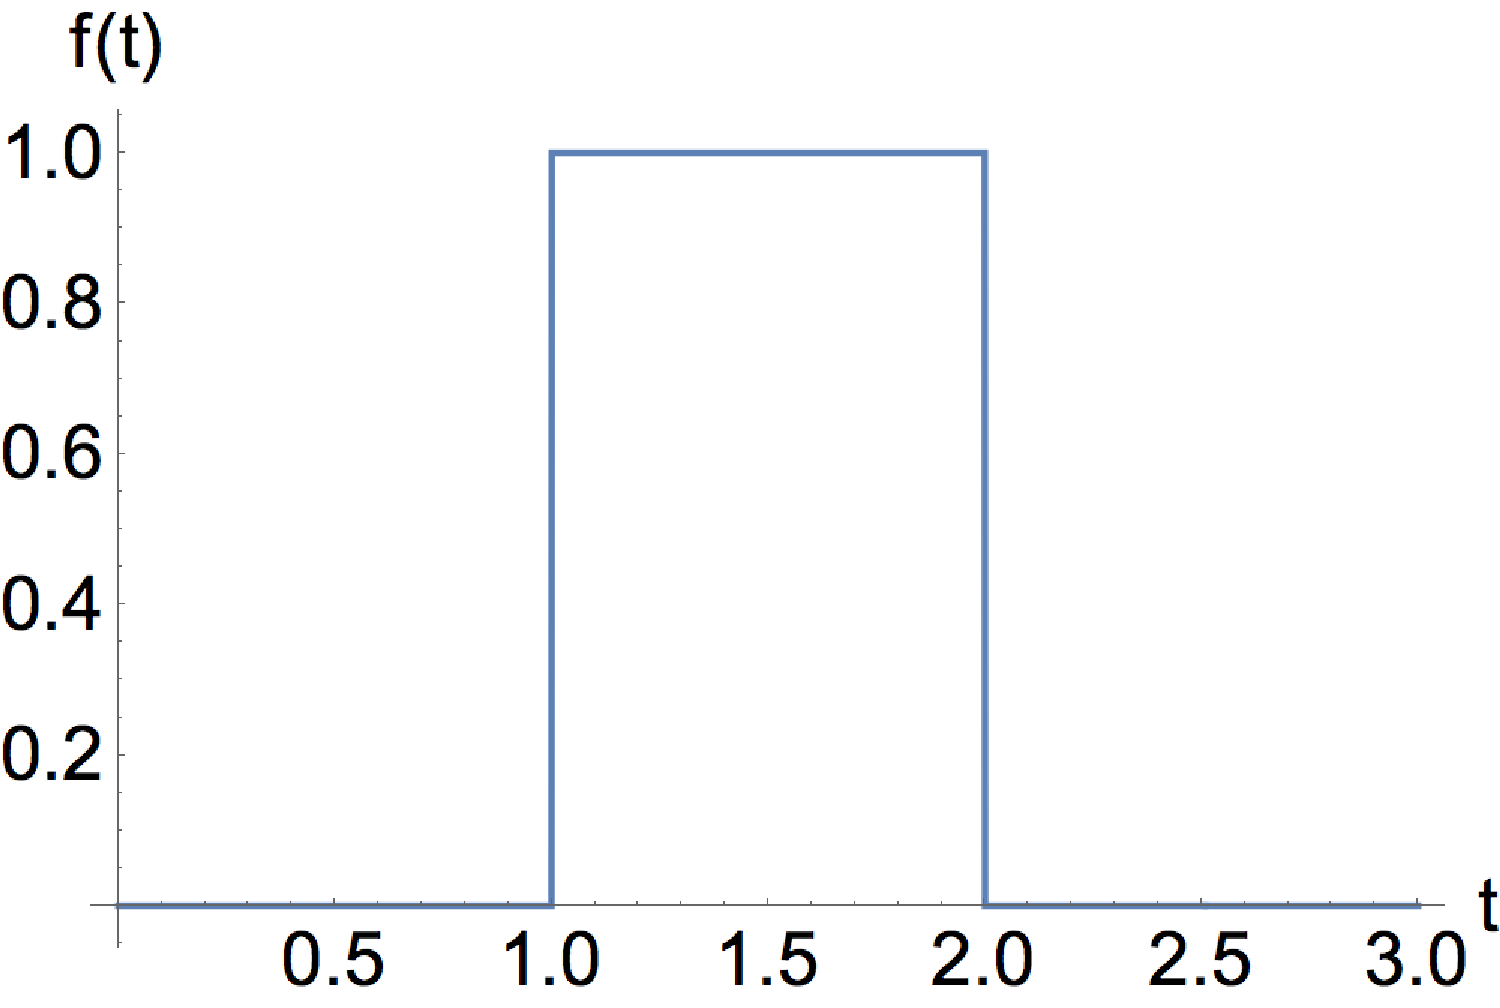
\includegraphics[scale=0.5]{pulse.png}

4. $\displaystyle \lap{U_\pi(t) cos(t-\pi)}$

\subsection*{Solution}
To check your answers, substitute $c=1$ and $s=2$ as appropriate.

1. \hash{yy}{39574c}

2. 0.0677

3. 0.0585

4. $7.470 \times 10^{-4}$




%%%%%%%%%%%%%%%%%%%%%%%%%%%%%%%%
\newpage
%%%%%%%%%%%%%%%%%%%%%%%%%%%%%%%%
\section{Inverse Laplace Transform}

\subsection*{Resources}
\begin{itemize}
    \item Video: \url{https://www.khanacademy.org/math/differential-equations/laplace-transform/properties-of-laplace-transform/v/inverse-laplace-examples} % 19m
\end{itemize}

\subsection*{Comment}
Being able to reversing the Laplace transform is a crucial skill required for applying it to solving ODE's. It can be a little confusing at first however, so I recommend to take your time to understand the essential steps involved thoroughly, as this will then give you greater confidence when you come to apply this to solving ODE's. To this end, the video listed in the resource is a fantastic introduction to this.

\subsection*{Challenge}
Determine the function $f(t)$ by finding the inverse of the following Laplace transforms:

1. $\displaystyle F(s)=\frac{1}{(s-1)^2}$

2. $\displaystyle F(s)=\frac{1-s}{s^2}$

3. $\displaystyle F(s)=\frac{2 e^{-2s}}{s^2-2s+2}$

4. $\displaystyle F(s)=\frac{6}{2+s^4}$

5. $\displaystyle F(s)=\frac{120+6s^3}{s^6}$

6. $\displaystyle F(s)=\frac{e^{12-3s}}{s-4}$


\subsection*{Solution}
To check your answers, substitute $t=2$ into your final answer. If there is a unit-step in your solution, precede your numerical answer with ``u(c)'' where ``c'' is the position of the unit step. So for example, an answer of $U_5 t^2$ would be entered as ``u(5.00)4.00'' (all numbers to two decimal places). An answer without a unit-step would just be entered to two decimal places (eg, ``4.00'' in the previous example).

1. Hash = 5cacdb\ldots

2. Hash = 41cf26\ldots

3. Hash = 45c11e\ldots

4. Hash = 9ffc7a\ldots

5. Hash = 766fd0\ldots

6. Hash = 6a7dc6\ldots




%%%%%%%%%%%%%%%%%%%%%%%%%%%%%%%%
\newpage
%%%%%%%%%%%%%%%%%%%%%%%%%%%%%%%%
\section{The Dirac delta function and its Laplace transform}

\subsection*{Resources}
\begin{itemize}
    \item Video I: \url{https://www.khanacademy.org/math/differential-equations/laplace-transform/properties-of-laplace-transform/v/dirac-delta-function}
    \item Video II: \url{https://www.khanacademy.org/math/differential-equations/laplace-transform/properties-of-laplace-transform/v/laplace-transform-of-the-dirac-delta-function}
\end{itemize}

\subsection*{Challenge}
Calculate the following Laplace transforms (treat $c$ as a positive constant):

1. $\displaystyle \lap{\delta(t)}$

2. $\displaystyle \lap{\delta(t-c)}$

3. $\displaystyle \lap{\delta(t-2) Cos(4 t)}$

4. $\displaystyle \lap{\delta(t) (t^2+10)}$

\subsection*{Solution}
To check your solution, set $s=1$, $c=2$ and $t=1$ as appropriate to check your answers.

1. \hash{zz}{ffef92}

2. \hash{aaa}{826784}

3. \hash{bbb}{f44448}

4. \hash{ccc}{4ca484}




%%%%%%%%%%%%%%%%%%%%%%%%%%%%%%%%
\newpage
%%%%%%%%%%%%%%%%%%%%%%%%%%%%%%%%
\section{The Dirac delta function and its inverse Laplace transform}

\subsection*{Challenge}
Calculate the following Laplace transform:

$\displaystyle \delta(t-2) Sin(2t)$

Calculate the following inverse Laplace transforms:

1. $\displaystyle e^{-2s} Sin(2)$

2. $\displaystyle e^{-2s} Sin(4)$

\subsection*{Solution}
To check your answer, substitute $t=1$ into the final expression and evaluate the part inside and outside of the Dirac delta function separately. So for example, if your answer is $\delta(t-2) (t^2+1)$, the expression inside the delta-function is $t-2$ and will evaluate to $-1.00$ while the expression outside of the delta-function is $t^2+1$ and will evaluate to $2.00$.

1. Inside delta function: \hash{ddd}{7cec9e}; Outside delta function: \hash{eee}{8147e6}

2. Inside delta function: \hash{fff}{033c55}; Outside delta function: \hash{ggg}{b1643a}




%%%%%%%%%%%%%%%%%%%%%%%%%%%%%%%%
\newpage
%%%%%%%%%%%%%%%%%%%%%%%%%%%%%%%%
\section{A forced spring}

\begin{itemize}
    \item The \textbf{four} videos starting at \url{https://www.khanacademy.org/math/differential-equations/laplace-transform/laplace-transform-to-solve-differential-equation/v/laplace-transform-to-solve-an-equation}
    \item A useful table of Laplace transforms: \url{http://tutorial.math.lamar.edu/pdf/Laplace_Table.pdf}
\end{itemize}

\section*{Comment}
Here you finally get the opportunity to practise solving ODE's using the powerful method of Laplace transformations. Please takes notes from all four videos listed in the resources section; they provide very useful examples of how to use this method, including related algebraic techniques that are commonly required to solve such challenges.

\subsection*{Challenge}
The spring equation you encountered in challenge \ref{sec:hooke} introduced you to the concept of oscillation of a mass on a spring. There, the equation to determine the displacement of the spring $y$ from its equilibrium position was $y''+y=0$, which yields a solution $y=C_1 Cos(t) + C_2 Sin(t)$. This is free oscillation without external damping or driving, and it will oscillate according to the cosine and sine sum for all time ($t$). It is also possible to add a forcing term to the equation by making it non-homogeneous, such as in the form

\begin{equation}
    y'' + 4y = 2 Cos(3t)
\end{equation}

Here the forcing varies with time $t$ in the form of a cosine wave.

Use the Laplace transform method to solve the ODE in the above equation given a starting displacement of zero and an initial velocity of zero. You may use the table of Laplace transforms in the resources to help you.

\subsection*{Solution}
Substitute $t=1$ to check your final solution: $y(t=1)=0.2295$.




%%%%%%%%%%%%%%%%%%%%%%%%%%%%%%%%
\newpage
%%%%%%%%%%%%%%%%%%%%%%%%%%%%%%%%
\section{An exponential function}

\subsection*{Challenge}
Solve

\begin{equation}
    y''+5y'+4y=100e^{-2t}
\end{equation}

for $y$. Since the algebra gets very messy, you may use the following equation to help you:
\begin{equation}
    \frac{s^2-7s+90}{(s+1)(s+2)(s+4)} = \frac{32}{s+1} - \frac{50}{s+2} + \frac{17}{s+4}
\end{equation}

\subsection*{Solution}
Substitute $t=1$ to check your final solution: $y(1)=5.32$.




%%%%%%%%%%%%%%%%%%%%%%%%%%%%%%%%
\newpage
%%%%%%%%%%%%%%%%%%%%%%%%%%%%%%%%
\section{A unit step}

\subsection*{Comment}
In past challenges we studied the Laplace transform for $U_c f(t-c)$. So if $f(t)=t$ we must evaluate for $f(t-c)=t-c$. In the challenge here, we effectively have $f(t)=1$ and since ``1'' doesn't depend on $t$, $t-c$ doesn't do anything to the ``function''.

This challenge is interesting because unlike previous challenges, it is the first challenge where we really have no other option but to use the Laplace transform method, and so you can appreciate its power. In this challenge, we have a 2nd-order homogeneous equation (unforced oscillation) until $t=5$ when we apply a constant force. You will find your answer leads to a constant oscillation. But how can it lead to a constant oscillation if we are constantly applying a force? Shouldn't the oscillation slowly increase in magnitude due to the energy that is being added to the system from the constant force being applied? The answer is of course no: we take just as much energy out of the system when the velocity is in the opposite direction to the force as we add to the system when the velocity is in the same direction as the applied force.

One important point to note is that the inverse Laplace transform of $e^{-cs} s^2/(s^2+a^2)$ is $\lap{U_c Cos(a[t-c])}$ (not $\lap{U_c Cos([at-c])}$).

\subsection*{Challenge}
Solve

\begin{equation}
    y''+2y=U_5
\end{equation}

for $y$, given initial conditions $y(0)=0$ and $y'(0)=0$. 

\subsection*{Solution}

$y(t=6)=0.42$

Note that for $t<5$, the solution is zero. This is because there was no initial velocity and no initial acceleration, so there was no motion until a forcing was applied in terms of a constant force of ``1'' from $t=5$. If either of these had been non-zero, we would have had a non-zero value for $t<5$!

Optionally, you can try setting the initial conditions to non-zero values to see the effect this has on the final solution.




%%%%%%%%%%%%%%%%%%%%%%%%%%%%%%%%
\newpage
%%%%%%%%%%%%%%%%%%%%%%%%%%%%%%%%
\section{A sudden impulse}

\subsection*{Comment}
Here the system is stationary until $t=5$ when, instead of applying a constant force, we ``kick'' the system to start the oscillation. Thus you should expect your answer to reflect physics such as this.

\subsection*{Challenge}
Solve

\begin{equation}
    y''+2y=\delta(t-5)
\end{equation}

for $y$, given initial conditions $y(0)=0$ and $y'(0)=0$. 

\subsection*{Solution}

$y(6)=0.698$

Note how we have a simple oscillation after $t=5$, and nothing before it.

%\chapter{Systems of ODE's}
%% NT: Ask to draw some examples
\section{Homogeneous vs non-homogeneous}

\subsection*{Comment}
\emph{The following notes were developed by Zachary S. Tseng at Pennsylvania State University, USA (\url{http://www.math.psu.edu/tseng/}). Included here with kind permission.}

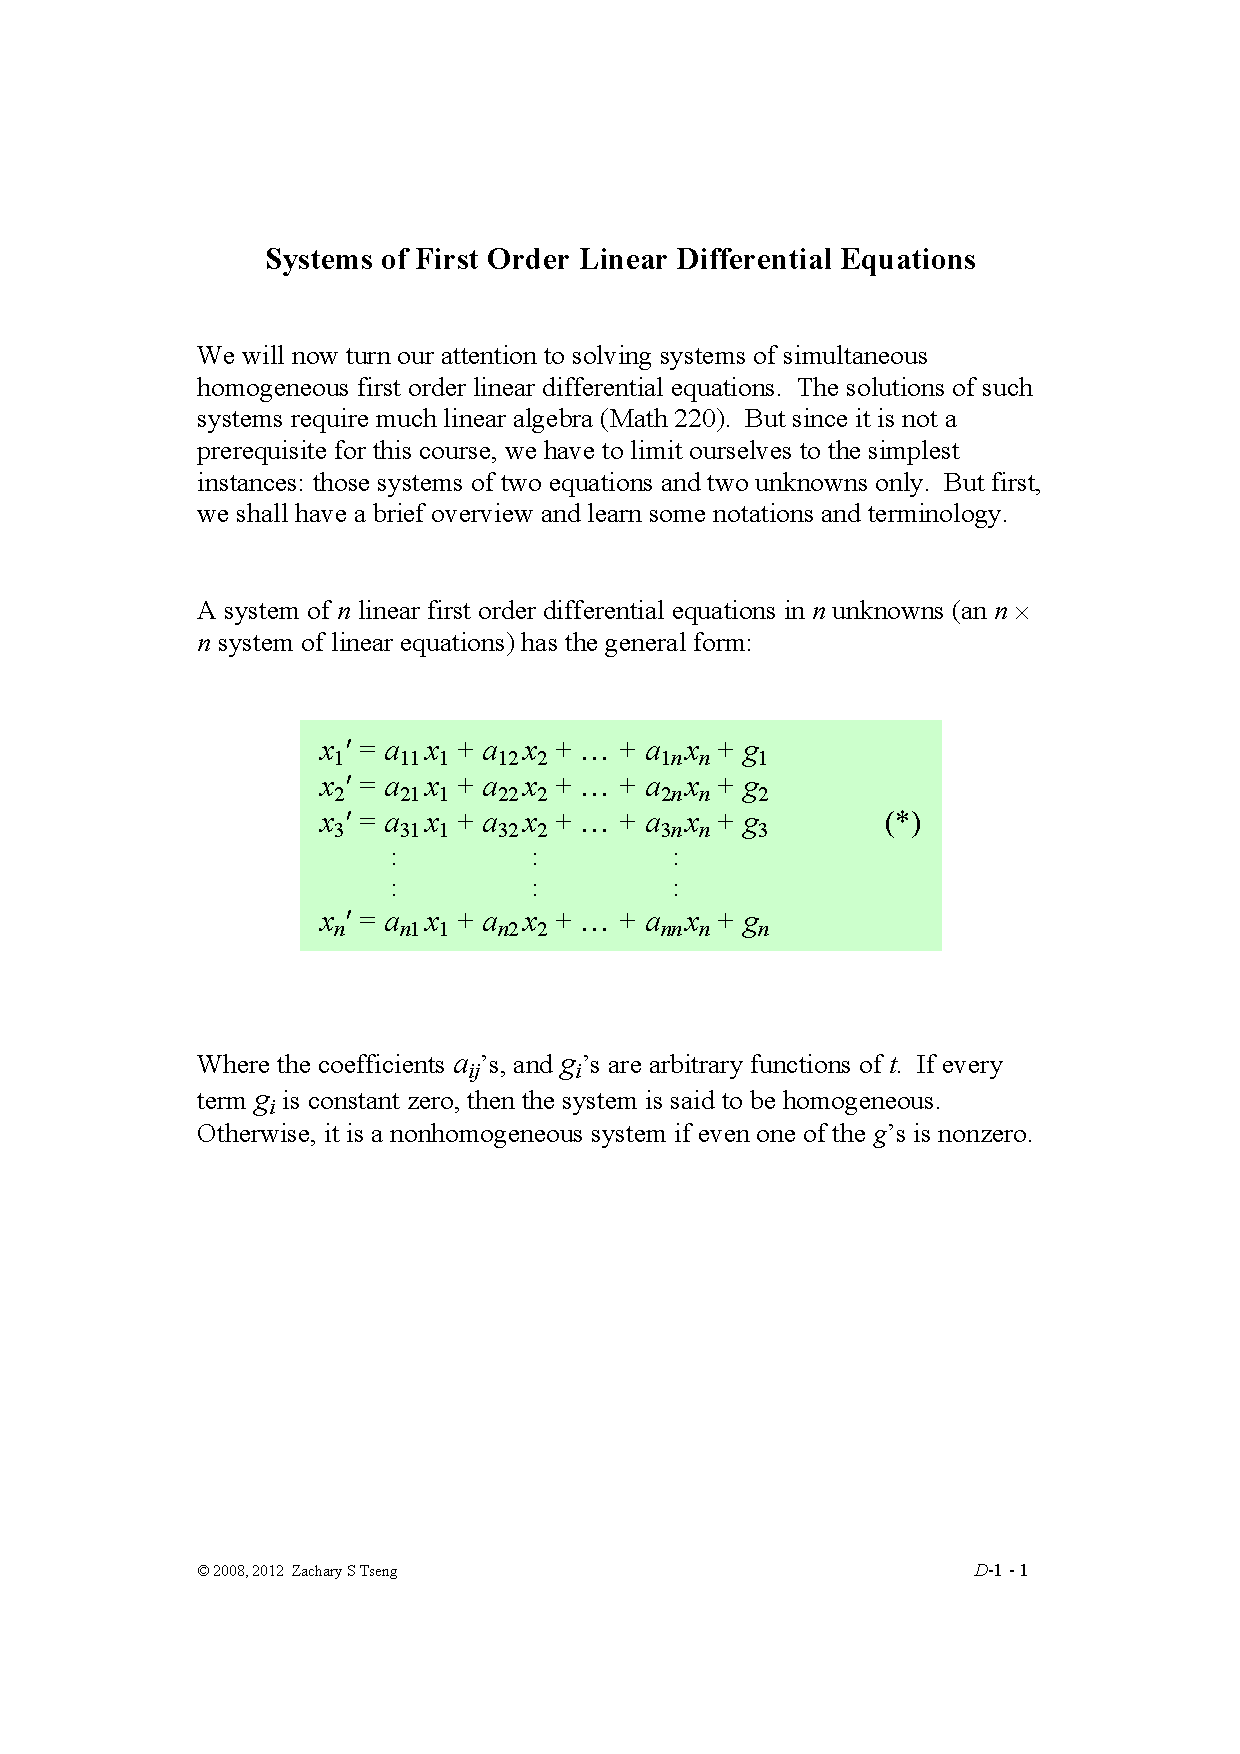
\includepdf[pages=-,pagecommand={},width=\textwidth,nup=1x1,frame=true]{External/systems_homo.pdf}

\subsection*{Challenge}
Separately add the points of the following \emph{homogeneous} and \emph{non-homogeneous} ODE systems:

1 point:
$\displaystyle
\left(
    \begin{array}{c}
        x_1' \\
        x_2' \\
        x_3'
    \end{array}
\right)
=
\left(
    \begin{array}{ccc}
        1 & 2 & 3 \\
        4 & 5 & 6 \\
        7 & 8 & 9
    \end{array}
\right)
\left(
    \begin{array}{c}
        x_1 \\
        x_2 \\
        x_3
    \end{array}
\right)
+
\left(
    \begin{array}{c}
        0 \\
        0 \\
        0
    \end{array}
\right)
$

2 points:
$\displaystyle
\left(
    \begin{array}{c}
        x_1' \\
        x_2' \\
        x_3'
    \end{array}
\right)
=
\left(
    \begin{array}{ccc}
        1 & 2 & 3 \\
        4 & 5 & 6 \\
        7 & 8 & 9
    \end{array}
\right)
\left(
    \begin{array}{c}
        x_1 \\
        x_2 \\
        x_3
    \end{array}
\right)
+
\left(
    \begin{array}{c}
        1 \\
        0 \\
        0
    \end{array}
\right)$

4 points:
$\displaystyle
\left(
    \begin{array}{c}
        x_1' \\
        x_2' \\
        x_3'
    \end{array}
\right)
=
\left(
    \begin{array}{ccc}
        1 & 2 & 3 \\
        4 & 5 & 6 \\
        7 & 8 & 9
    \end{array}
\right)
\left(
    \begin{array}{c}
        x_1 \\
        x_2 \\
        x_3
    \end{array}
\right)
+
\left(
    \begin{array}{c}
        1 \\
        \sin(t) \\
        0
    \end{array}
\right)$

8 points:
$\displaystyle
\left(
    \begin{array}{c}
        x_1' \\
        x_2' \\
        x_3'
    \end{array}
\right)
=
\left(
    \begin{array}{ccc}
        1 & 2 & 3 \\
        4 & 5 & 6 \\
        7 & 8 & 9
    \end{array}
\right)
\left(
    \begin{array}{c}
        x_1 \\
        x_2 \\
        x_3
    \end{array}
\right)
+
\left(
    \begin{array}{c}
        1 \\
        \sin(t) \\
        \tan(t)
    \end{array}
\right)$

\subsection*{Solution}
\textbf{Homogeneous}\\
\solint{h}{346b81}

\textbf{Non-homogeneous}\\
\solint{i}{773ffc}




%%%%%%%%%%%%%%%%%%%%%%%%%%%%%%%%
\newpage
%%%%%%%%%%%%%%%%%%%%%%%%%%%%%%%%
\section{Basis for creating a system of equations from a single homogeneous ODE}
\label{sec:systembasis}

\subsection*{Resources}
\begin{itemize}
    \item Pages 1-4 of the PDF \url{http://www.math.psu.edu/tseng/class/Math251/Notes-LinearSystems.pdf} 
\end{itemize}

\subsection*{Comment}
\emph{Note that the notation $y^{(2)}$ means ``the 2nd differential of y'' while the notation $y^2$ (without the brackets around the $2$) means ``y-squared''.}

Considering the general form of an nth-order linear equation,
\begin{equation}
    a_n y^{(n)} + a_{n-1} y^{(n-1)} + \cdots + a_1 y^{(1)} + a_0 y = g(t)
\end{equation}
we substitute $x_1=y$, $x_2=y'$, \ldots, $x_n=y^{(n-1)}$ and $x_n'=y^{(n)}$.

When replacing a $y$-term by an $x$ term, the $n$ in $x_n$ corresponds to one more than the number of times $y$ is differentiated. So $x_{n+1}$ corresponds to $y$ being differentiated $n$ times and similarly $x_n$ corresponds to $y$ being differentiated $n-1$ times.

Note that $x_n'$ is one more differential than $x_n$, so $x_n'$ corresponds to $(y^{(n-1)})' = y^{(n)}$.
So the $n$ in $x_n'$ corresponds to the number of times $y$ is differentiated (ie, $y^{(n)}$).

To understand how this helps us write high-order ODE's as a system of equations, consider the equation
\begin{equation}
    y''' - 2y'' + 3y' - 4y = 0
\end{equation}

First re-write the ODE in terms of $x$ and $x'$. Note that there is no ``$x_0'$'' so we just write it as $x_1$ in both equations.
\begin{align}
    x_4 - 2 x_3 + 3 x_2 - 4 x_1 &= 0 \label{eq:xs} \\
    x_3' - 2 x_2' + 3 x_1' - 4 x_1 &= 0 \label{eq:xprimes}
\end{align}

Our aim is to write the system of equations in the form $\bm{x'} = \bm{A}\bm{x}$. Note that there is no ``$x_4'$'' in our equations, so the largest value of $n$ in $x_n'$ will be 3 (ie, $x_3'$). So we can write
\begin{equation}
    \left(
        \begin{array}{c}
            x_1' \\
            x_2' \\
            x_3'
        \end{array}
    \right)
    =
    \left(
        \begin{array}{ccc}
            ? & ? & ? \\
            ? & ? & ? \\
            ? & ? & ?
        \end{array}
    \right)
    \left(
        \begin{array}{c}
            x_1 \\
            x_2 \\
            x_3
        \end{array}
    \right)
\end{equation}
where the question marks are values that we have to find.

By direct comparison of equations \ref{eq:xs} and \ref{eq:xprimes} we know that $x_1' = x_2$ which can be written as $x_1' = 0 x_1 + 1 x_2 + 0 x_3$ yielding the first line in the matrix $\bm{A}$:
\begin{equation}
    \left(
        \begin{array}{c}
            x_1' \\
            x_2' \\
            x_3'
        \end{array}
    \right)
    =
    \left(
        \begin{array}{ccc}
            0 & 1 & 0 \\
            ? & ? & ? \\
            ? & ? & ?
        \end{array}
    \right)
    \left(
        \begin{array}{c}
            x_1 \\
            x_2 \\
            x_3
        \end{array}
    \right)
\end{equation}

We can then proceed to do $x_2$ in a similar fashion:
\begin{equation}
    \left(
        \begin{array}{c}
            x_1' \\
            x_2' \\
            x_3'
        \end{array}
    \right)
    =
    \left(
        \begin{array}{ccc}
            0 & 1 & 0 \\
            0 & 0 & 1 \\
            ? & ? & ?
        \end{array}
    \right)
    \left(
        \begin{array}{c}
            x_1 \\
            x_2 \\
            x_3
        \end{array}
    \right)
\end{equation}

In order to express $x_3'$ in the above matrix form, we need it in terms of $x_1$, $x_2$ and $x_3$ rather than $x_4$, so instead of direct comparison, we swap $x_4$ for $x_3'$ in equation \ref{eq:xs} to read
\begin{equation}
    x_3' - 2 x_3 + 3 x_2 - 4 x_1 = 0
\end{equation}
and then isolate $x_3'$ to read $x_3' = 4 x_1 - 3 x_2 + 2 x_3$ yielding the final form of our systems of equations
\begin{equation}
    \left(
        \begin{array}{c}
            x_1' \\
            x_2' \\
            x_3'
        \end{array}
    \right)
    =
    \left(
        \begin{array}{ccc}
            0 & 1 & 0 \\
            0 & 0 & 1 \\
            4 & -3 & 2
        \end{array}
    \right)
    \left(
        \begin{array}{c}
            x_1 \\
            x_2 \\
            x_3
        \end{array}
    \right)
\end{equation}

Note that this is only considering a homogeneous equation. If it is non-homogeneous, you will have an extra term in the final step and will need a matrix of the form  $\bm{x'} = \bm{A}\bm{x} + \bm{g}$ as shown in the answer to exercise 4(b) on page 5 of the PDF.

So why do we want to do this? Well, notice that in this example we started with a complicated 3rd-order ODE and reduced it into 3 1st-order ODE's. Similarly, if we started with a 2nd-order ODE, we could reduce the equation to 2 1st-order ODE's. In general, for an nth-order ODE we can reduce it to $n$ 1st-order ODE's. If we can then learn how to solve simultanious sets of 1st-order ODE's, we have a powerful method of increasing our understanding (and even solving) difficult higher-order ODE's. 

Similarly, if you are given a system of 2 1st-order ODE's, you can know that it can form a single 2nd-order ODE. 

\subsection*{Challenge}
Write the following ODE's in matrix form:

1) $2y'' + 4y' - 6y = 0$

2) $y'' - 4y' + 5y = 0$

\subsection*{Solutions}
To check your answers, sum the values of all the terms in your matrix $\bm{A}$.

1) 2

2) 0




%%%%%%%%%%%%%%%%%%%%%%%%%%%%%%%%
\newpage
%%%%%%%%%%%%%%%%%%%%%%%%%%%%%%%%
\section{Systems of equations from a non-homogeneous ODE}

\section*{Comment}
The approach is very similar when you have a non-homogeneous ODE, but you just have to remember to add the forcing term at the end. For example, considering an equation similar to before, but this time with a cosine forcing term:

\begin{equation}
    y''' - 2y'' + 3y' - 4y = \cos t
\end{equation}

We have

\begin{align}
    x_4 - 2 x_3 + 3 x_2 - 4 x_1 &= \cos t \\
    x_3' - 2 x_2' + 3 x_1' - 4 x_1 &= \cos t
\end{align}

By comparison we still have $x'_1 = x_2$ and $x'_2 = x_3$ but now when we replace $x_4$ with $x'_3$ and re-arrange we have
\begin{equation}
   x_3' = \cos t + 4 x_1 - 3 x_2 + 2 x_3
\end{equation}

leading to a final system of equations of the form

\begin{equation}
    \left(
        \begin{array}{c}
            x_1' \\
            x_2' \\
            x_3'
        \end{array}
    \right)
    =
    \left(
        \begin{array}{ccc}
            0 & 1 & 0 \\
            0 & 0 & 1 \\
            4 & -3 & 2
        \end{array}
    \right)
    \left(
        \begin{array}{c}
            x_1 \\
            x_2 \\
            x_3
        \end{array}
    \right)
    +
    \left(
        \begin{array}{c}
            0 \\
            0 \\
            \cos t
        \end{array}
    \right)
\end{equation}

\subsection*{Challenge}
Re-write the following differential equations as a system of first-order differential equations:

1) $y'' + y' + y = \cos t$

2) $y'' - 5 y' + 9 y = t \cos 2t$

\subsection*{Solutions}
Please compare your solution with that of your partner or ask the teacher.



%%%%%%%%%%%%%%%%%%%%%%%%%%%%%%%%
\newpage
%%%%%%%%%%%%%%%%%%%%%%%%%%%%%%%%
%\input{matrices}
\section{Matrices}

\subsection*{Resources}
\begin{itemize}
    \item PDF: Pages 6-17 of the PDF \url{http://www.math.psu.edu/tseng/class/Math251/Notes-LinearSystems.pdf}
\end{itemize}

\subsection*{Comment}
It is worth spending some time getting comfortable with manipulating matrices, since this is an indispensable basis for the work that is about to follow. The PDF gives a quick introduction to matrices. For a more thorough introduction, the Khan Academy playlist on linear algebra [1] is excellent, although beyond the scope of this course.

One note to deal with any confusion arising with regard to eigenvectors with matrices with zeros. For $(A-rI)$ equal to something like
\begin{equation}
\left(
    \begin{array}{cc}
        0 & 0 \\
        1 & 2
    \end{array}
\right)
\end{equation}
the top row can be ignored since any $x_1$ and $x_2$ will satisfy the top row.

Similarly, for a case such as
\begin{equation}
\left(
    \begin{array}{cc}
        2 & 0 \\
        2 & 0
    \end{array}
\right)
\end{equation}
you will have
\begin{align}
    2 x_1 + 0 x_2 &= 0 \\
    2 x_1 &= 0 \\
    x_1 &= 0
\end{align}
which is satisfied by
\begin{equation}
\left(
    \begin{array}{c}
        0 \\
        1
    \end{array}
\right)
\end{equation}
(where the $1$ could in principle be any number, but is the minimum integer that satisfies the condition.)

Finally, note that $(A-rI) = ((a, b), (c, d))$ will give you two equivalent formulas $a x_1 + b x_2 = 0$ and $c x_1 + b x_2 = 0$, even if they may appear different on first glance. If you want, you can prove to yourself that they are the same by multiplying the bottom row by $a/c$.

\vspace{0.2cm}
\noindent [1] \url{https://www.khanacademy.org/math/linear-algebra/alternate-bases}

\emph{The following notes were developed by Zachary S. Tseng at Pennsylvania State University, USA (\url{http://www.math.psu.edu/tseng/}). Included here with kind permission.}

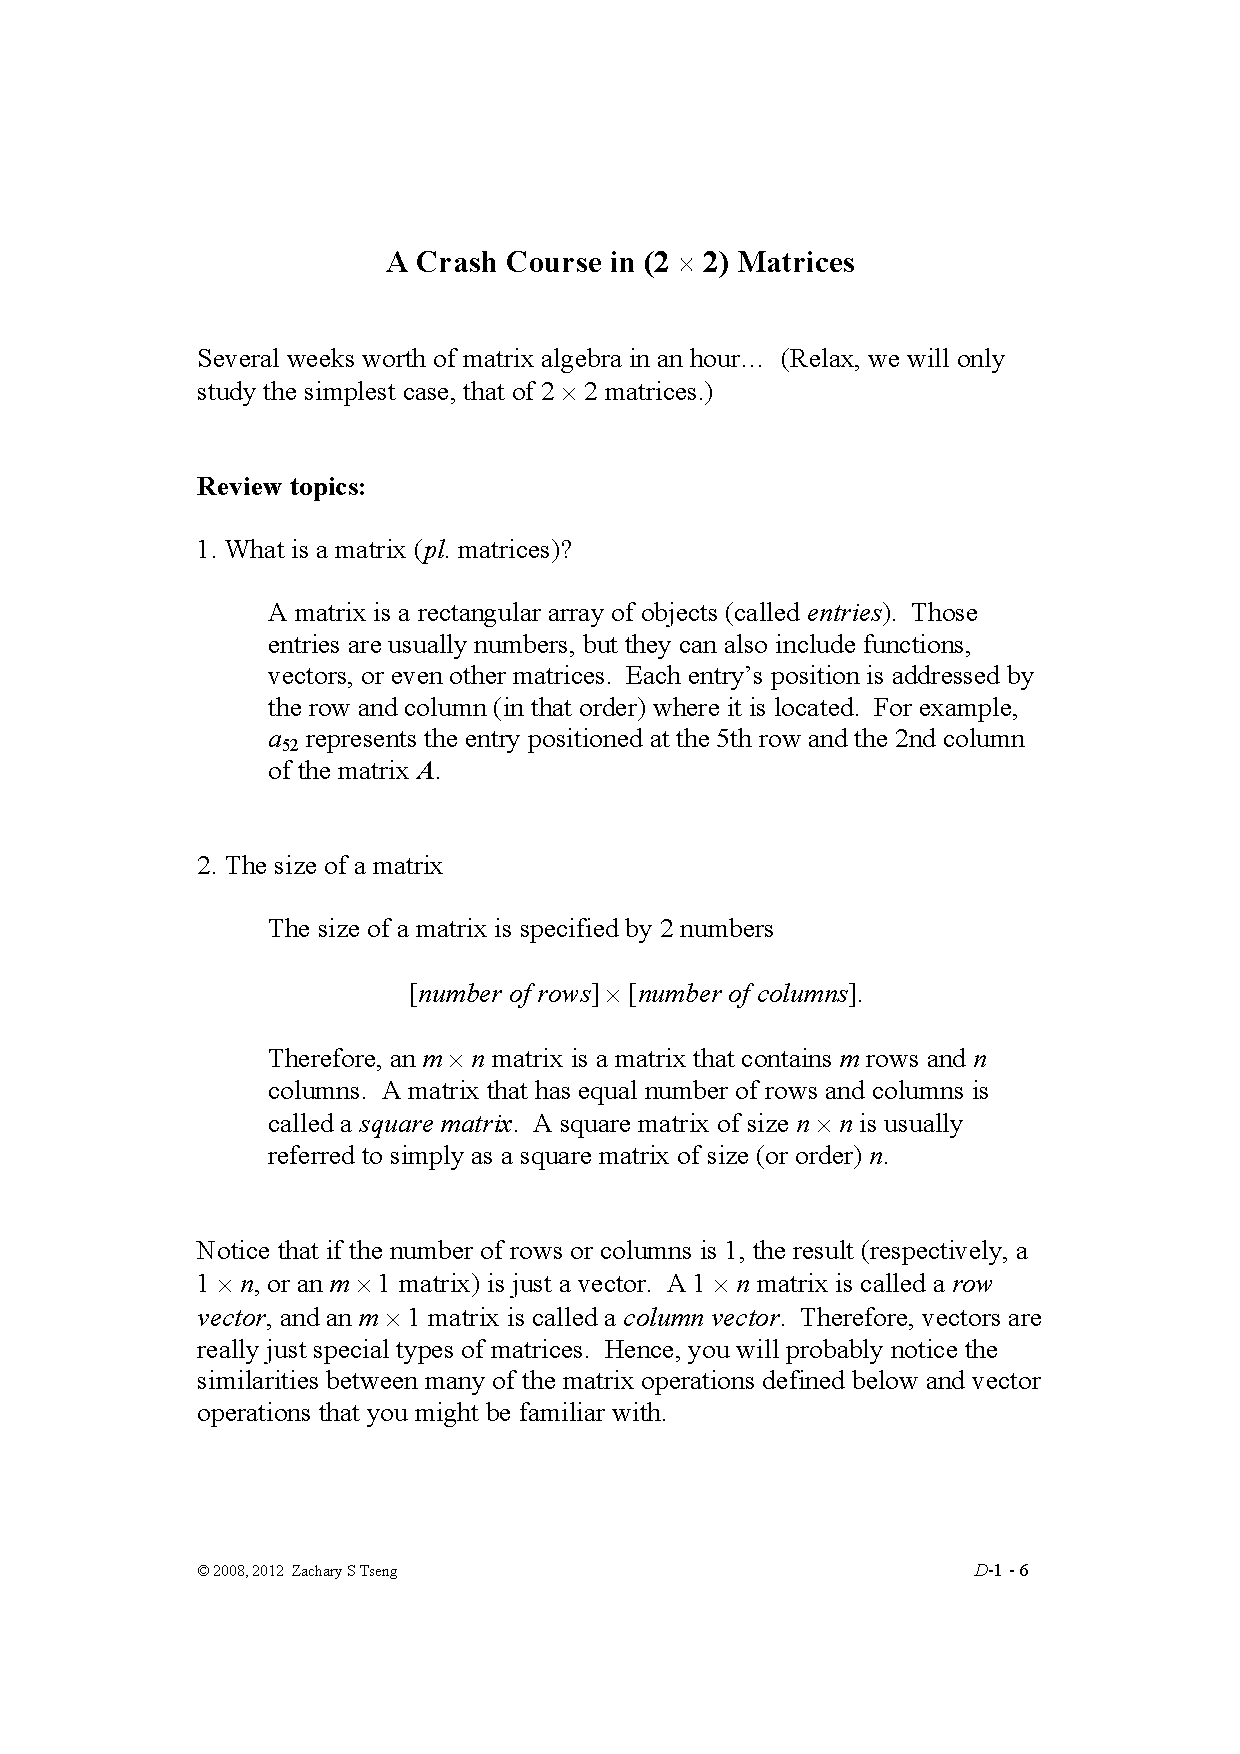
\includepdf[pages=-,pagecommand={},width=\textwidth,nup=1x1,frame=true]{External/matrices.pdf}

\subsection*{Challenges}
Considering the matrices
$\displaystyle
    \mathbf{C} =
\left(
    \begin{array}{cc}
        -5 & -1 \\
        7 & 3
    \end{array}
\right)
$
and
$\displaystyle
    \mathbf{D} =
\left(
    \begin{array}{cc}
        2 & 0 \\
        -2 & -1
    \end{array}
\right)
$
calculate:

1. $\mathbf{C} + 2 \mathbf{D}$

2. $\mathbf{C} \mathbf{D}$

3. $\mathbf{D} \mathbf{C}$

4. $\det(\mathbf{CD})$

5. $\mathbf{(CD)}^{-1}$

6. Find the eigenvectors and eigenvalues of $\mathbf{C}$

7. Find the eigenvectors and eigenvalues of $\mathbf{D}$

\subsection*{Solutions}
1. The sum of the terms in the matrix should be $2$.

2. The sum of the terms in the matrix should be $-2$.

3. The sum of the terms in the matrix should be $-10$.

4. $16$

5. The sum of the terms in the matrix should be $-5/4$.

6. Eigenvalues 2 and -4 will have eigenvectors $(s,-7s)$ and $(s,-s)$ respectively where $s$ is any non-zero number.

7. Eigenvalues 2 and -1 will have eigenvectors $(s,-2s/3)$ and $(0,s)$ respectively where $s$ is any non-zero number.


%%%%%%%%%%%%%%%%%%%%%%%%%%%%%%%%
\newpage
%%%%%%%%%%%%%%%%%%%%%%%%%%%%%%%%
\section{Eigenvector equivalence}

\subsection*{Comment}
Considering the matrix
\begin{equation}
    A = \left(
        \begin{array}{cc}
            1 & 2 \\
            -3 & -4
        \end{array}
    \right)
\end{equation}
The eigenvalues are -2 and -1. Considering the eigenvalue -2, 
\begin{equation}
    A - Ir = \left(
        \begin{array}{cc}
            3 & 2 \\
            -3 & -2
        \end{array}
    \right)
\end{equation}
To determine the eigenvector we can either take the top or bottom row in the calculation $(A - Ir)x = 0$.
The top and bottom row appear with different numbers but it is easy to see that they yield multiples of the same eigenvector and are therefore equivalent.

Complex eigenvectors are no different, but it can sometimes be hard to see that they are indeed equivalent.

\subsection*{Challenge}
Show that the equation $(A - Ir)\bm{x} = {0}$, where
\begin{equation}
     A-Ir = \left(
        \begin{array}{cc}
            -3 -3i & 6 \\
            -3 & 3-3i
        \end{array}
    \right)
\end{equation}
yields the same eigenvector, irrespective of whether you calculate the eigenvector using the top or bottom row of $(A-Ir)$. You may find that one of the representations of the eigenvectors looks like $(1-i,1)$.

\subsection*{Solutions}
You should be able to generate two eigenvectors by using the top and bottom rows of the $A-Ir$ matrix, and show that they are in fact the same eigenvector by multiplying by an equivalent (imaginary) number. Please discuss with your partner or the teacher in class if you have trouble.



%%%%%%%%%%%%%%%%%%%%%%%%%%%%%%%%
\newpage
%%%%%%%%%%%%%%%%%%%%%%%%%%%%%%%%
\section{Solving systems of ODE's}
\label{sec:systemsolving}

\subsection*{Comment}
When decomposing a higher-order ODE into a system of 1st-order ODE's, we are actually dealing with a special form of 1st-order ODE system that looks like

\begin{equation}
    \label{eq:hightoloworder}
     \left(
        \begin{array}{c}
            x_1' \\ x_2' \\ x_3' \\ x_4'
        \end{array}
    \right)
    =
     \left(
        \begin{array}{cccc}
            0 & 1 & 0 & 0 \\
            0 & 0 & 1 & 0 \\
            0 & 0 & 0 & 1 \\
            -a_5/a_1 & -a_4/a_1 & -a_3/a_1 & -a_2/a_1
        \end{array}
    \right)
     \left(
        \begin{array}{c}
            x_1 \\ x_2 \\ x_3 \\ x_4
        \end{array}
    \right)
    +
     \left(
        \begin{array}{c}
            0 \\ 0 \\ 0 \\ f(y)
        \end{array}
    \right)
\end{equation}

which naturally arise from a higher-order ODE like
\begin{equation}
    a_1 y'''' + a_2 y''' + a_3 y'' + a_4 y' + a_5 y = f(y)
\end{equation}

This can be considered in terms of other phenomena however whereby the system of ODE's cannot be expressed as a higher-order ODE. In this challenge you can learn about such systems.

\emph{The following notes were developed by Zachary S. Tseng at Pennsylvania State University, USA (\url{http://www.math.psu.edu/tseng/}). Included here with kind permission.}

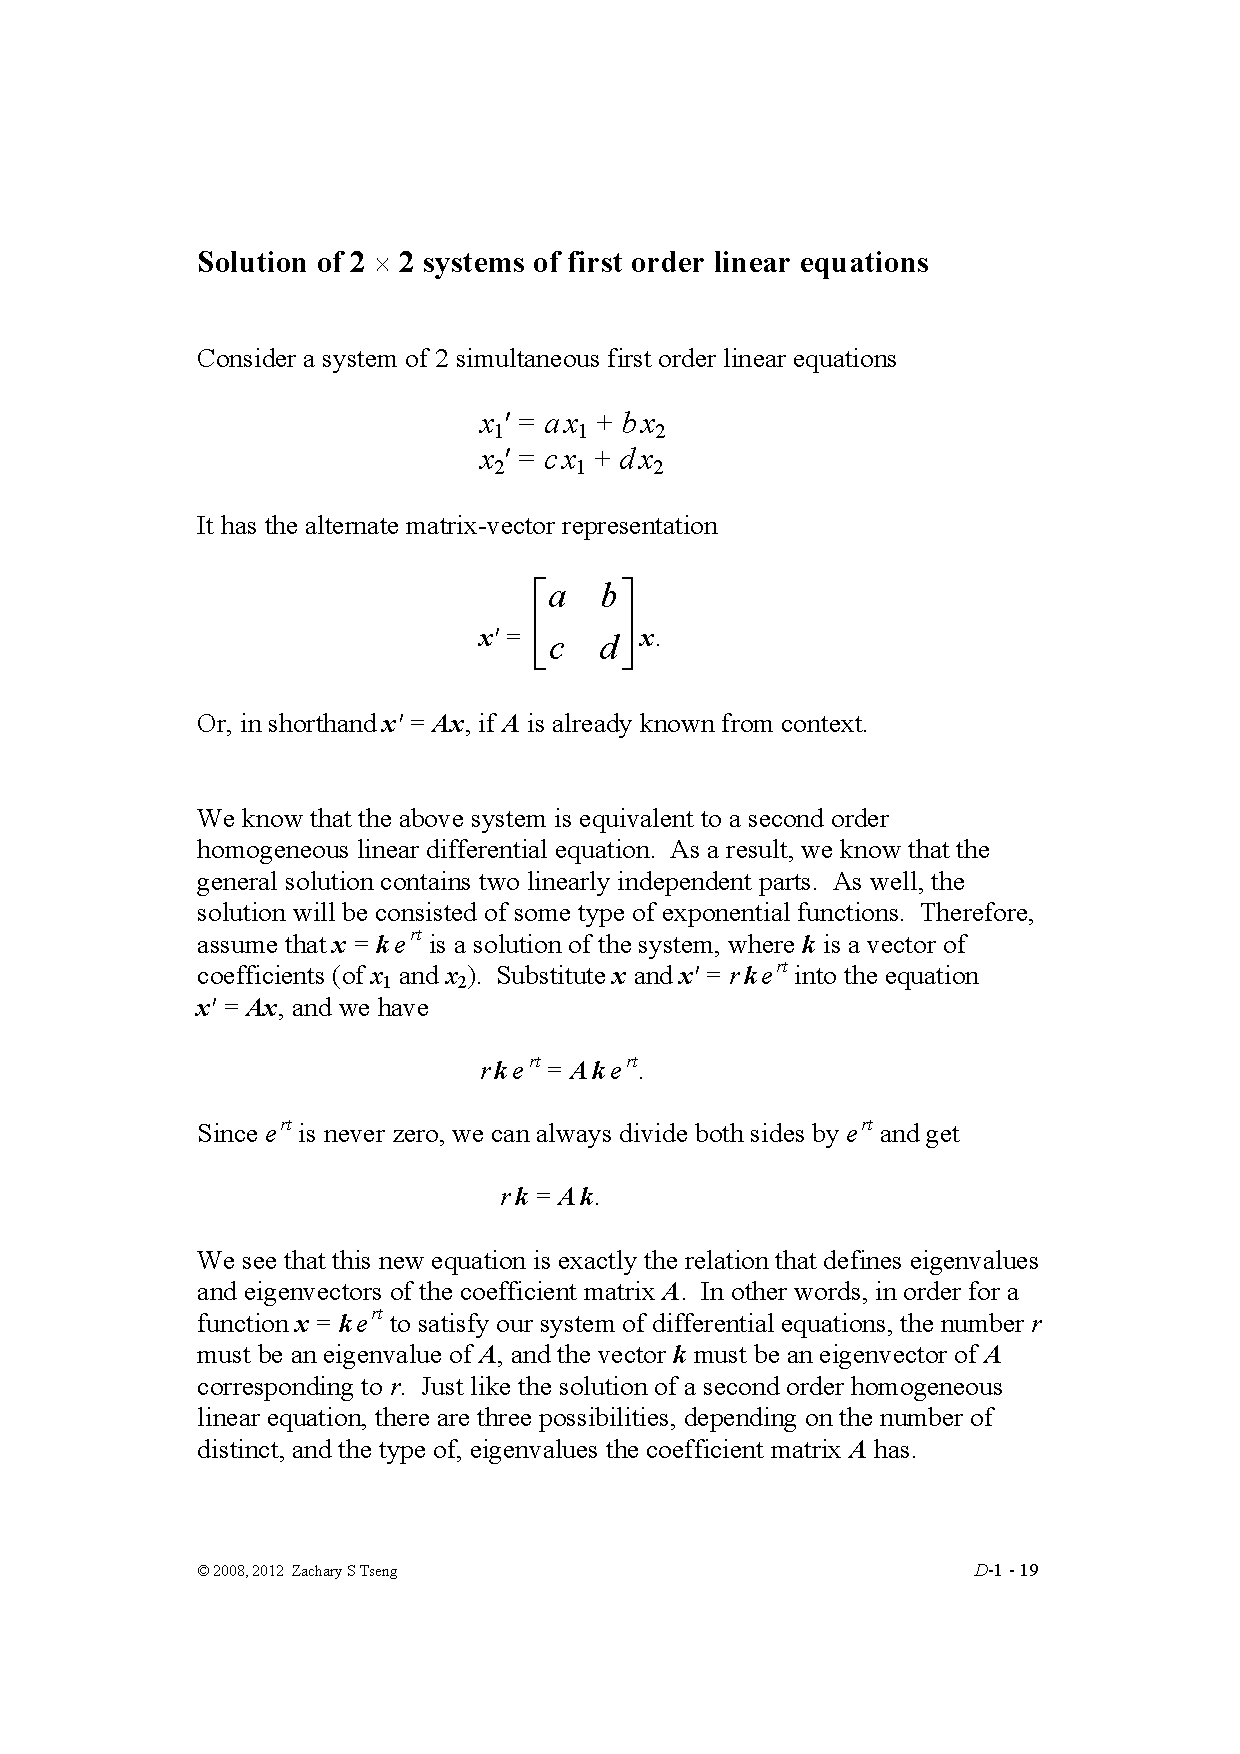
\includepdf[pages=-,pagecommand={},width=\textwidth,nup=1x1,frame=true]{External/linear_systems.pdf}

\subsection*{Challenge}
\label{sec:systemsolvingchallenges}
Answer questions 2, 3 and 4 in the last page in the notes above.

\subsection*{Solutions}
It might not be clear to you why solutions involve vectors and what this means physically, but for now, please just get used to solving equations in this fashion.

Solutions can be found in the Appendix \ref{sec:systemsolvingsols}.


%NT: Add something about intersection of graphs? https://en.wikipedia.org/wiki/System_of_linear_equations
% Good resources: http://www.math.psu.edu/tseng/class/Math251/




%%%%%%%%%%%%%%%%%%%%%%%%%%%%%%%%
\newpage
%%%%%%%%%%%%%%%%%%%%%%%%%%%%%%%%
\section{Solving systems of ODE's with initial conditions}
\label{sec:systemsolvinginit}

\subsection*{Challenge}
\label{sec:systemsolvinginitchallenges}
Continuing from the previous challenge, solve the problems 8, 9 and 10 in the PDF resource above, using initial conditions as given.

\subsection*{Solutions}
You should find that you solution is consistent with

8. $\displaystyle \bm{x}(0.8) = \matrixcrr{-1.90}{-0.66}$

9. $\displaystyle \bm{x}(0.8) = \matrixcrr{33100}{-13300}$

10. $\displaystyle \bm{x}(0.8) = \matrixcrr{-1.71}{1.96}$



%%%%%%%%%%%%%%%%%%%%%%%%%%%%%%%%
\newpage
%%%%%%%%%%%%%%%%%%%%%%%%%%%%%%%%
\section{Graphs of system solutions}

\subsection*{Resources}
In challenge \ref{sec:systembasis} you considered systems of equations that arose from decomposition of a higher-order ODE into a system of 1st-order ODE's as depicted in equation \ref{eq:hightoloworder}. For a 2nd-order ODE, for example, you could decompose this into two 1st-order ODE's, determining $x_1$ and $x_2$ with solutions such as
\begin{equation}
    \label{eq:en6tet}
    \bm{x} = \matrixcrr{x_1}{x_2} = c_1 \matrixcrr{-1}{6} e^{-6t} + c_2 \matrixcrr{1}{1} e^t
\end{equation}

or written another way:
\begin{align}
    x_1 &= -c_1 e^{-6t} + c_2 e^t \label{eqn:sysgraphx1} \\
    x_2 &= 6 c_1 e^{-6t} + c_2 e^t \label{eqn:sysgraphx2} 
\end{align}

This particular system arose from a 2nd-order differential equation:
\begin{equation}
    y'' + 5y' - 6y = 0 \label{eqn:sys2ndoode}
\end{equation}

We have learned in challenge \ref{sec:systembasis} that this 2nd-order equation can be written in terms of $x$:

\begin{equation}
    x_3 + 5x_2 - 6 x_1 = 0
\end{equation}

Thus we remember that $x_1 = y$ and $x_2 = y'$, allowing equations \ref{eqn:sysgraphx1} and \ref{eqn:sysgraphx2} to be written as
\begin{align}
    y &= -c_1 e^{-6t} + c_2 e^t \label{eqn:syspos} \\
    y' &= 6 c_1 e^{-6t} + c_2 e^t \label{eqn:sysvel} 
\end{align}

Perhaps, for example, the original 2nd-order ODE (equation \ref{eqn:sys2ndoode}) represented the position of an atom on an axis with respect to time. Then equation \ref{eqn:syspos} represents position at time $t$ while equation \ref{eqn:sysvel} represents the velocity (or more commonly, when multiplied by the mass, represents the momentum).

Thus the graph represents the variation of momentum (velocity) with position, called the ``phase-space'' of the system. A specific trajectory can be followed given boundary conditions that determine the starting condition. For example, if the particle at time $t=0$ is known to have position $y=1$ and velocity $y'=2$ we can impose the boundary condition
\begin{equation}
    \bm{x}(0) = \matrixcrr{1}{2}
\end{equation}
to determine the coefficients $c_1$ and $c_2$ and obtain a unique trajectory.

We can then plot the phase-space for various boundary conditions. In the graph below, we show examples where $c_1 = c_2 = \{0, 0.5, 1, 1.5, 2\}$:

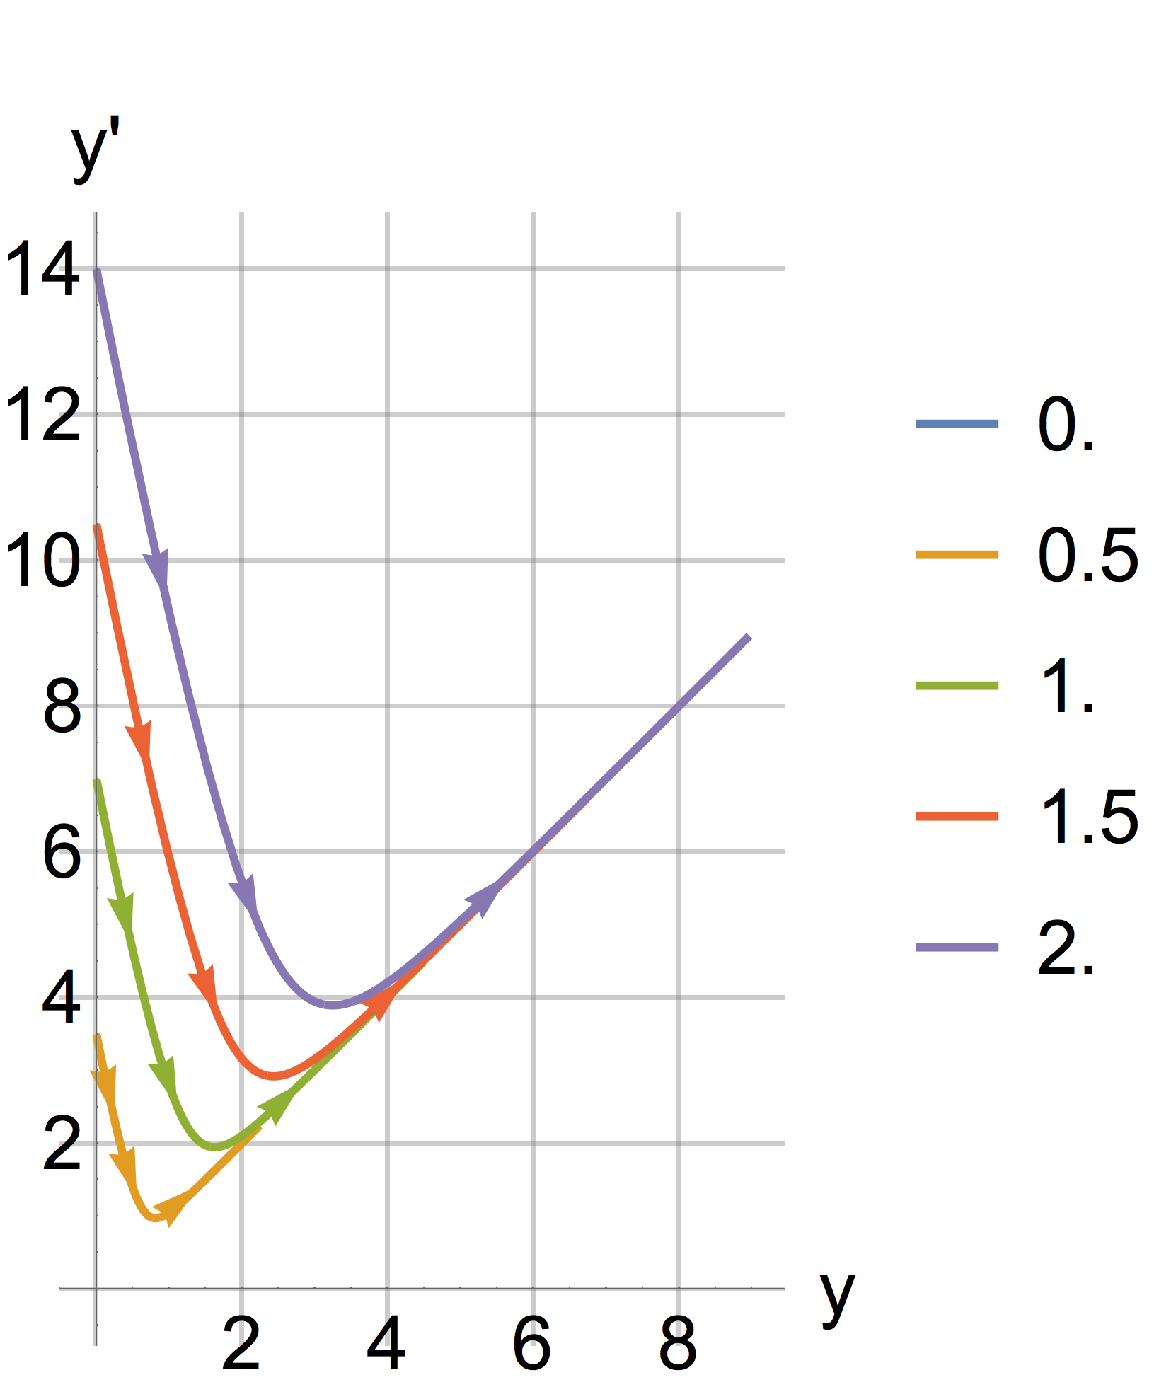
\includegraphics[scale=0.7]{phase_space_1.png}

You can note that as $t$ increases, the term $e^{-6t}$ goes to zero leaving the $e^t$ dominant, and since this features in both $y$ and $y'$, you get $y \propto y'$ for large $t$. % NT: Check this: As expected for this negatively-damped equation, both the velocity and position increase rapidly with time.

The examples we are considering here are relatively simple, however this can be used to identify complex and chaotic phenomena visually. For example, considering a pendulum gently swinging backwards and forwards, it is possible to trace out the phase-space as shown here:

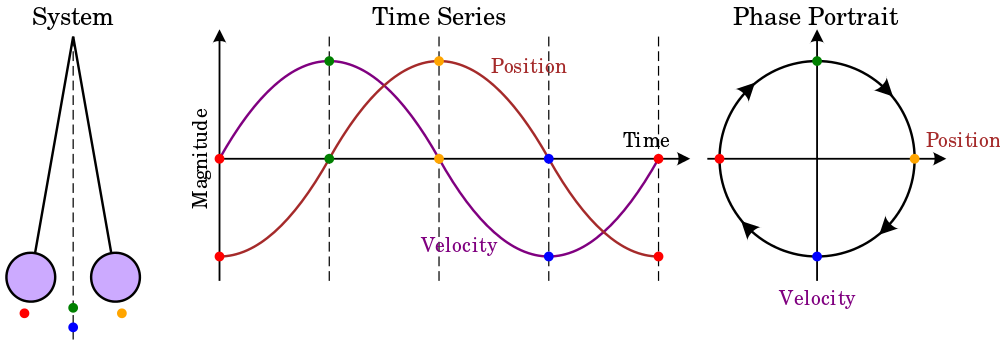
\includegraphics[scale=0.4]{pendulum_gentle.png}\\
\emph{\small{Source: \url{https://commons.wikimedia.org/wiki/File:Pendulum_phase_portrait_illustration.svg}, Wikipedia user Krishnavedala}}

If you increase the speed of the pendulum, at some critical point, instead of swinging back to the original position it will start whirring round and round. Expressed in terms of vertical angle and angular velocity, the graph becomes:

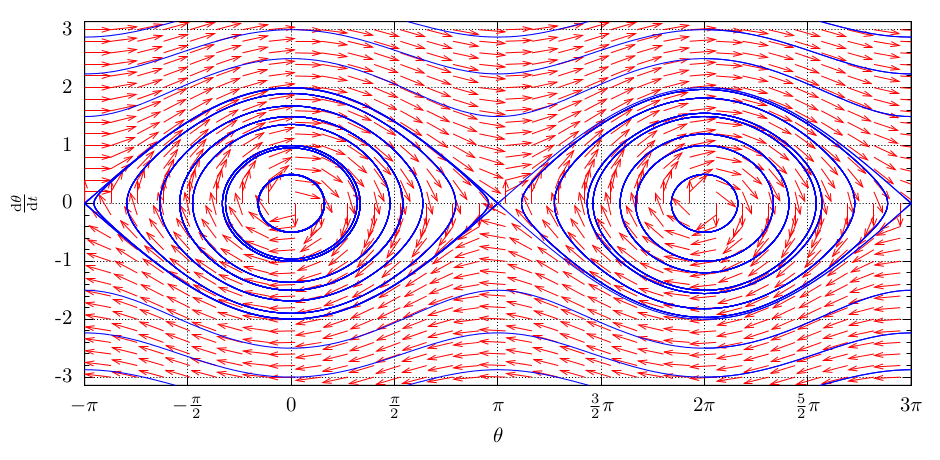
\includegraphics[scale=1]{pendulum_fullphase.png}\\
\emph{\small{Source: \url{https://commons.wikimedia.org/wiki/File:Pendulumphase.png}}}

At low velocities the pendulum swings back and forth (blue circles, angular velocity both positive and negative), but at high velocities, the angular velocity stays positive (or negative) and the pendulum whirs round and round in one direction (blue wavy lines). Note that position $\theta = \pi$ is when the rigid pendulum is pointing exactly upwards. So with no momentum it is stationary here, albeit unstable, because with a tiny velocity it will perform a full loop, slowing (but not stopping) as it reaches the top again.

\subsection*{Challenge}
1.\\
Considering the graph shown earlier of angular momentum vs angle for a rigid pendulum, add the points of the following true statements:

\textbf{1 point} An initial angular velocity of 1 unit results in whirring circular motion irrespective of the starting angle.

\textbf{2 points} An initial angular velocity of -2.5 units results in whirring circular motion irrespective of the starting angle.

\textbf{4 points} An initial angle of $\pi/2$ combined with an angular velocity of 1 unit results in periodic swinging motion.

\textbf{8 points} An initial angle of $\pi/2$ combined with an angular velocity of 1 unit results in circular whirring motion.

\textbf{16 points} An initial angle of $0$ combined with an angular velocity of 0 units results in periodic swinging motion.

\textbf{32 points} An initial angle of $0$ combined with an angular velocity of 0 units results in a stationary system.

\textbf{64 points} An initial angle of $\pi$ combined with an angular velocity of 0 units results in a stationary system.

\textbf{128 points} An initial angle of $\pi/2$ combined with an angular velocity of 0 units results in a stationary system.

\textbf{256 points} An initial angular velocity of 3 units results in whirring circular motion in the same direction as an initial angular velocity of -3 units.

\textbf{512 points} An initial angular velocity of 3 units results in whirring circular motion in the opposite direction as an initial angular velocity of -3 units.

% NT: Split this into its own challenge
2.\\
For equations that do not necessarily derive from a higher-order ODE, the $x$ and $y$ axes do not necessarily represent position-momentum phase-space, and the exact meaning of the axes depends on the specific system under study.

In challenge \ref{sec:systemsolving} you determined general solutions to exercises 2, 3 and 4.
The example earlier in this challenge (equation \ref{eq:en6tet}) corresponds to exercise 1 of that same page.

The graphs below correspond to systems arising from exercises 1 to 5.
Place the graphs below in the same order those exercises.
Note that in order to maintain clarity, the graphs are not necessarily plotted over the same time interval $t$, but they do all start at $t=0$.

\begin{tabular}{cc}
    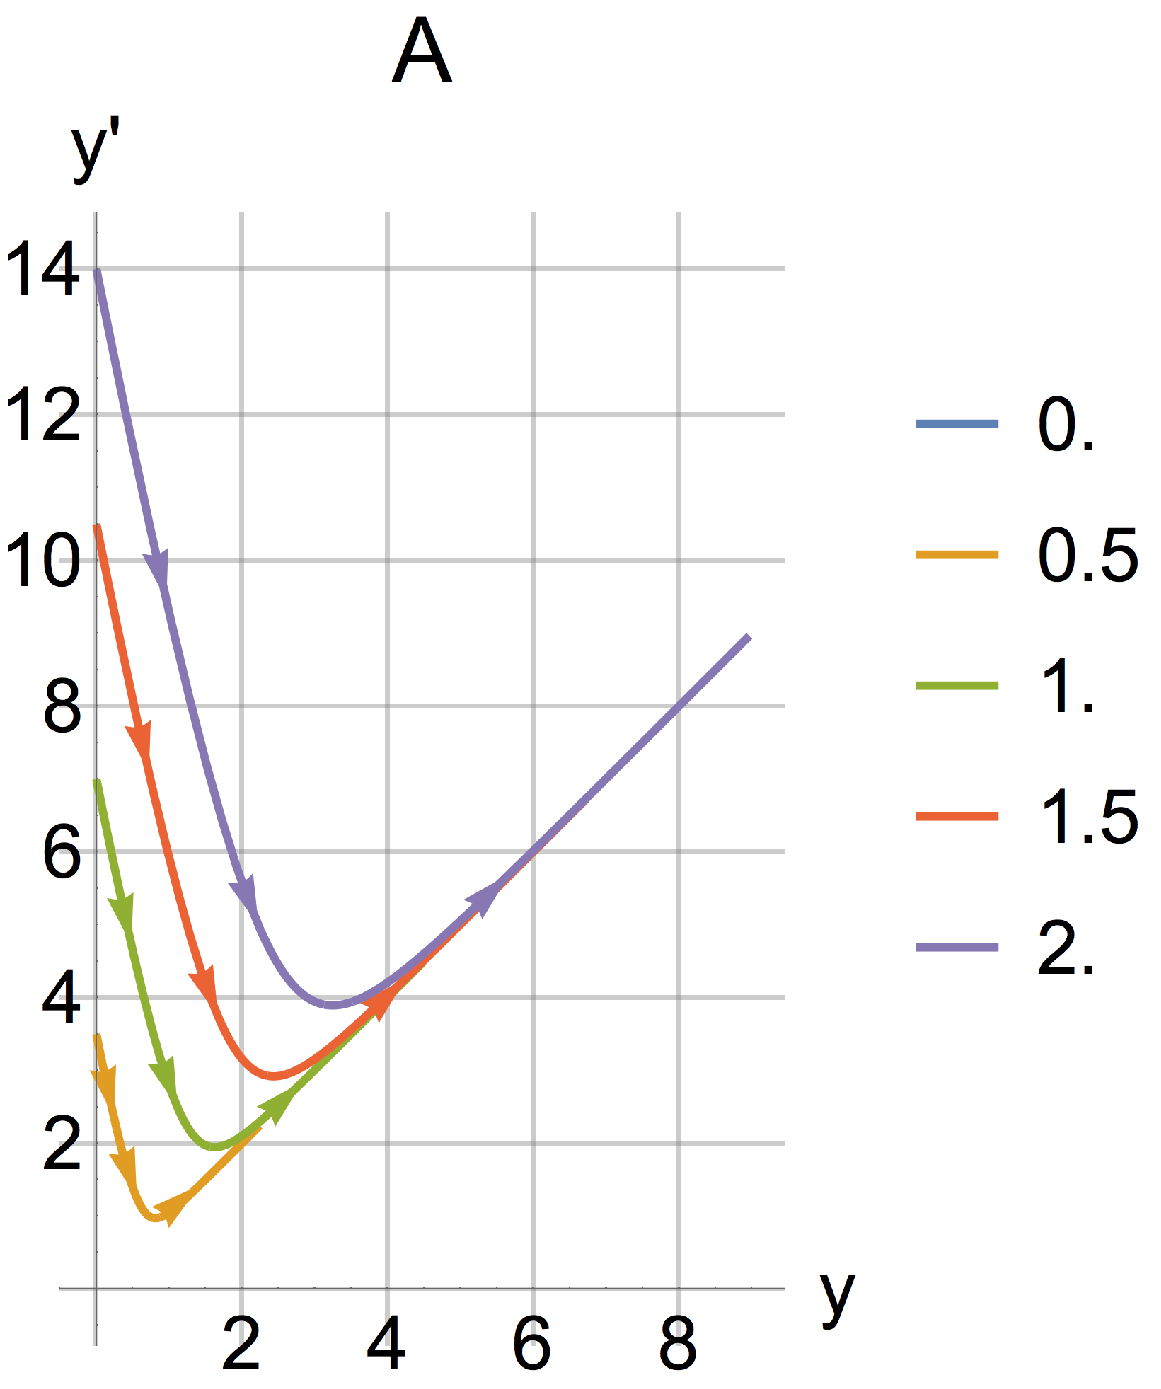
\includegraphics[scale=0.6]{phase_space_a.png} &
    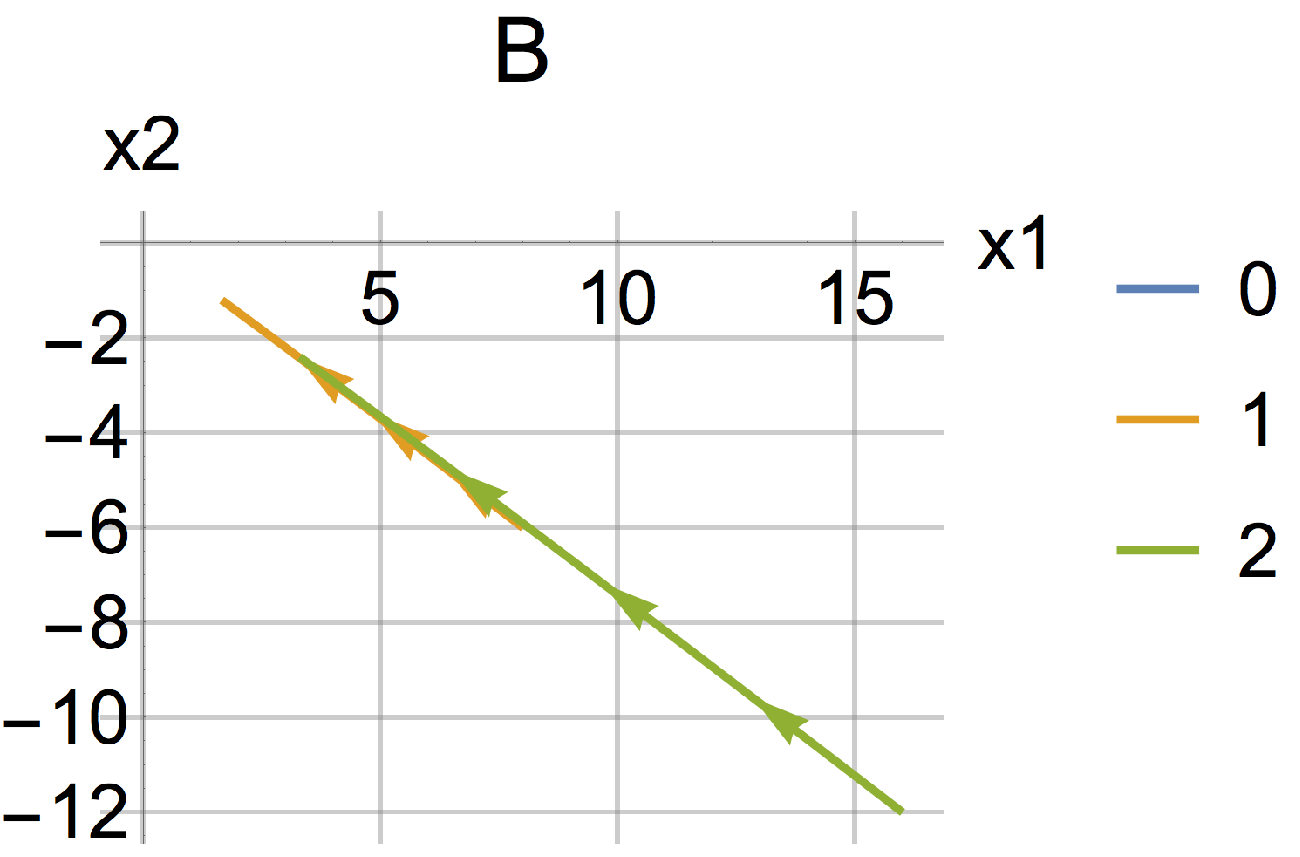
\includegraphics[scale=0.6]{phase_space_b.png} \\
    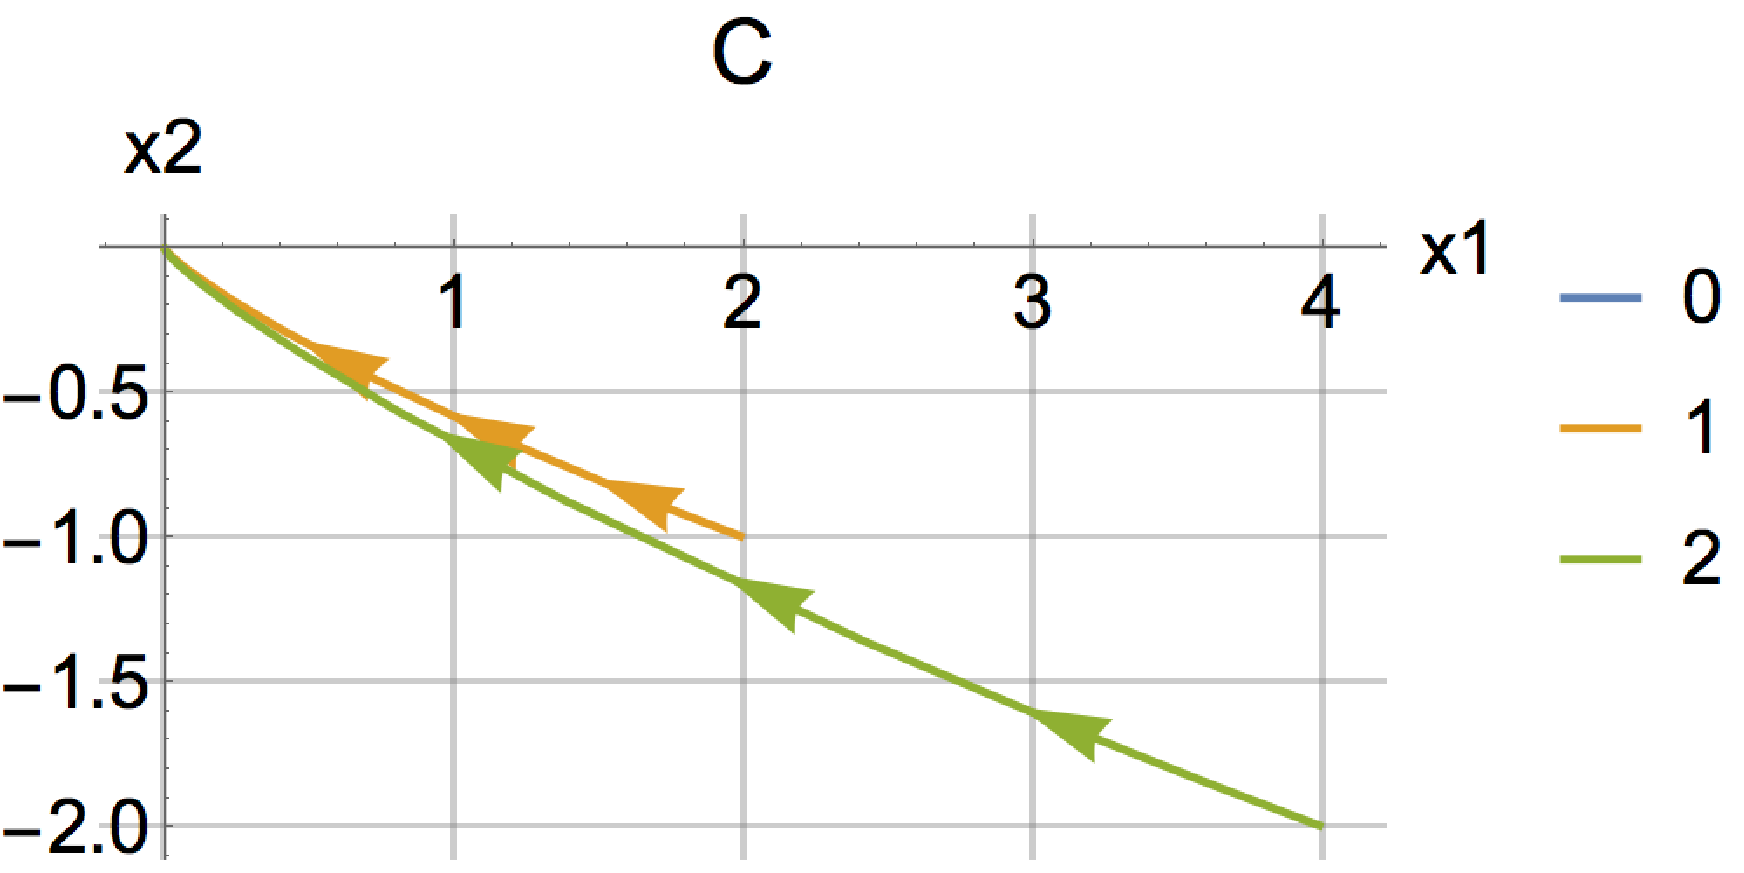
\includegraphics[scale=0.6]{phase_space_c.png} &
    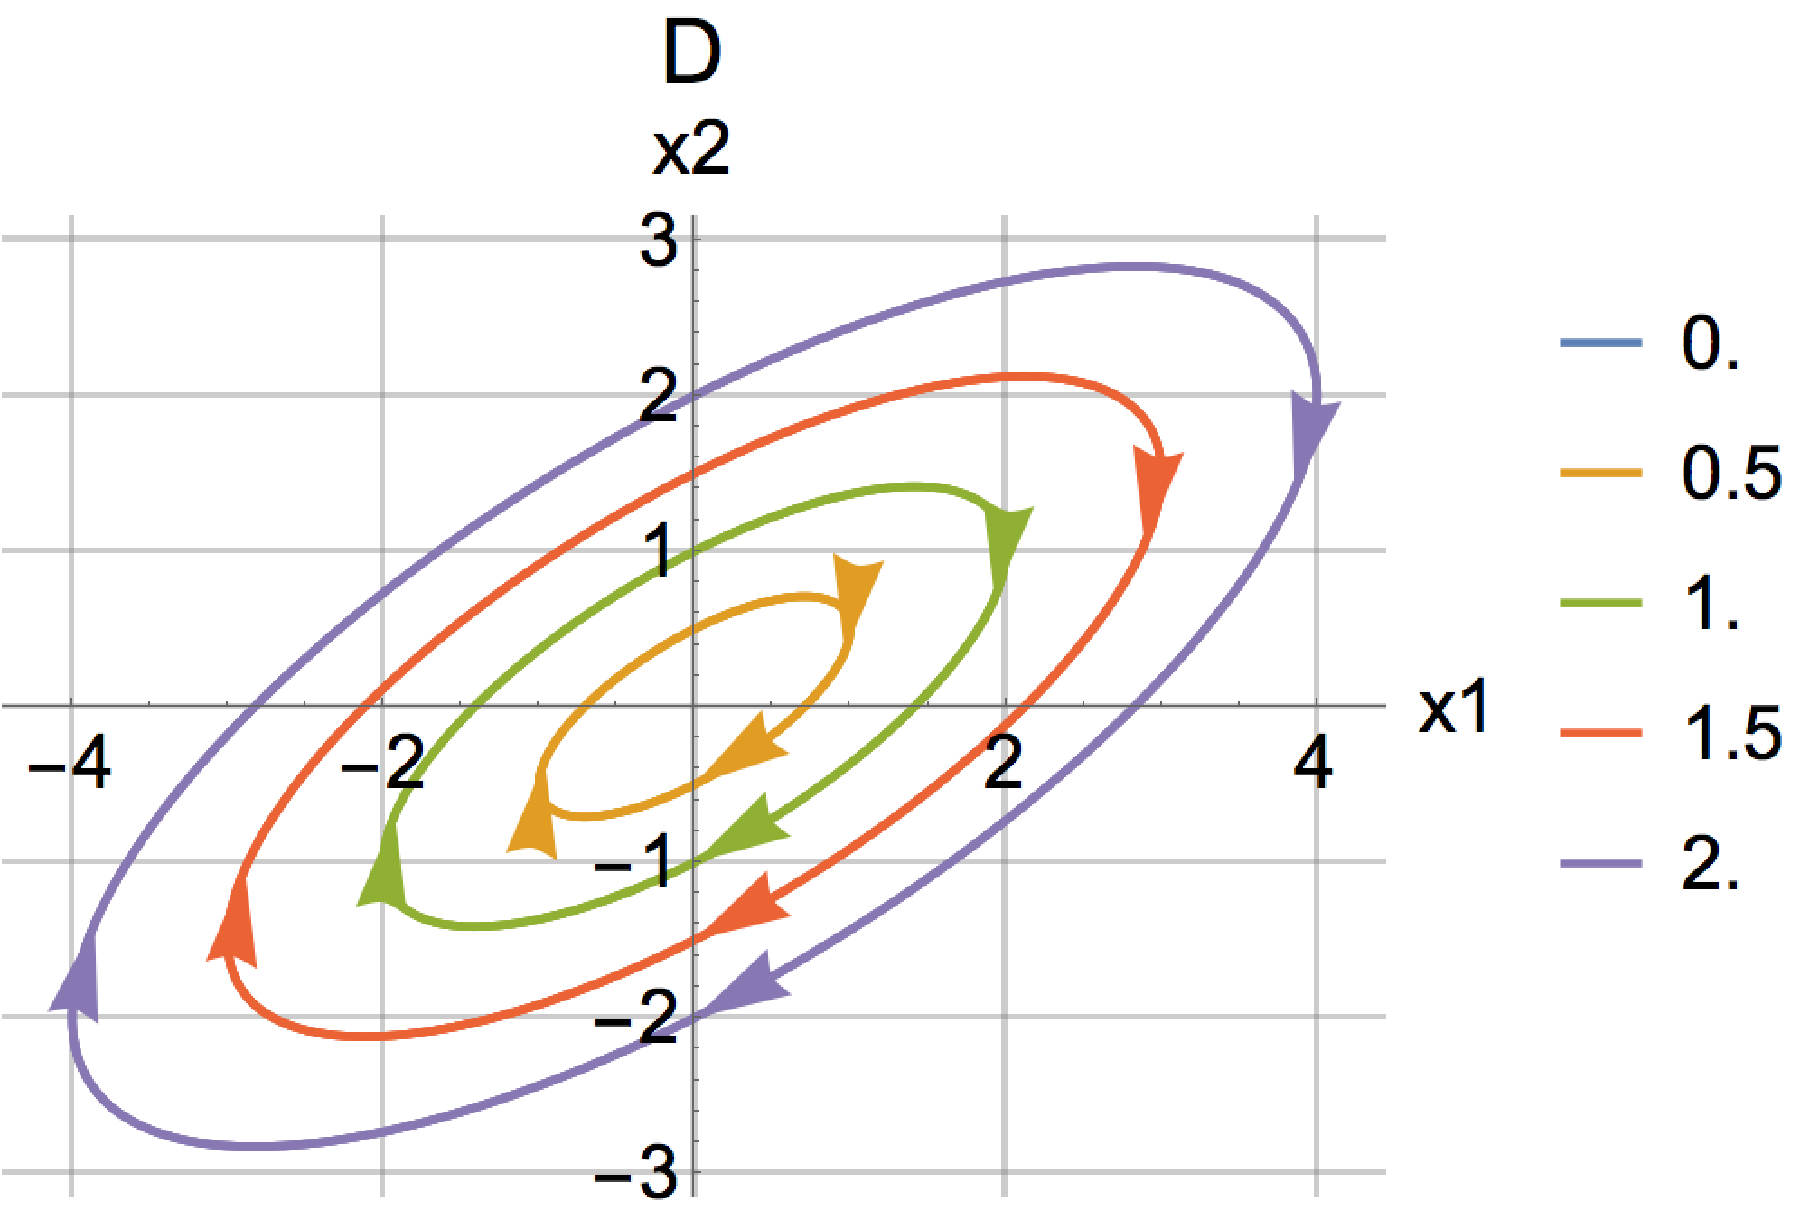
\includegraphics[scale=0.5]{phase_space_d.png} \\
    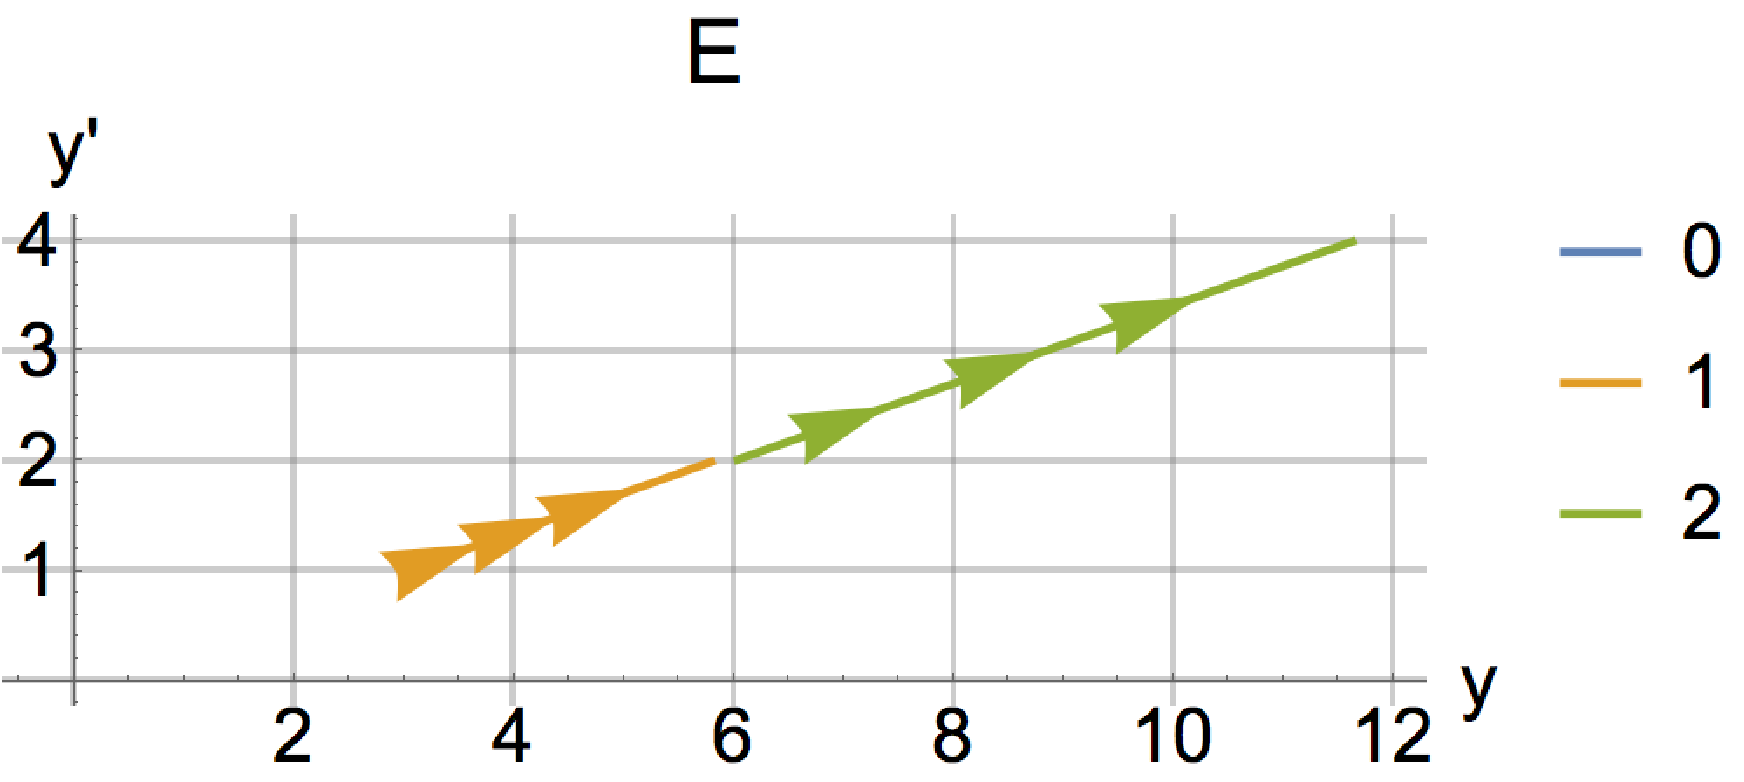
\includegraphics[scale=0.6]{phase_space_e.png} &
\end{tabular}
% NT: Add graphs that have the same starting position so students need to check the shape of the graph, as well as the t=0 position

\subsection*{Solutions}
1.\\
\solint{k}{5f8194}

2.\\
\solstr{j}{b63166}


% NT: bifurcation? https://en.wikipedia.org/wiki/Hopf_bifurcation
% Other Pendulum resources of interest: http://math.stackexchange.com/questions/666806/nonlinear-pendulum and https://www.youtube.com/watch?v=6KSXLGHsrrs

%\chapter{Numerical methods}
%\section{System set-up}

\subsection*{Comment}
Numerical methods of solving ODE's are common. Here we will consider Euler and Runge-Kutta approaches.

\subsection*{Challenge}

Considering the following ODE:

\begin{equation}
    \dot{v} = g - v^2
\end{equation}

1. Sketch a direction field to show the behaviour of solutions to this ODE. In particular, what values of $v$ will lead to stable solutions?

2. What type of ODE is this?

\subsection*{Solutions}
1. (Stable)\\
\soltwodp{a}{4ac0c3}

1. (Unstable)\\
\soltwodp{b}{9ed192}

2. Please compare your solution with your partner or ask the teacher.




%%%%%%%%%%%%%%%%%%%%%%%%%%%%%%%%
\newpage
%%%%%%%%%%%%%%%%%%%%%%%%%%%%%%%%
\section{Tangent lines}

\subsection*{Resource}
\begin{itemize}
    \item Chapter 3: \url{https://raw.githubusercontent.com/kriskissel/ConceptsODE/master/main.pdf}
\end{itemize}

\subsection*{Challenge}
1. Given that $y(t)$ satisfies the equation $y' = y^3 + 3t$ subject to $y(1) = 2$, find $y'(1)$ without solving the differential equation and obtain the equation of the tangent to the curve $y(t)$ at the point (1,2).

2. Use the tangent line to estimte the value at $t = 1.5$.

\subsection*{Solution}
2. $7.5$




%%%%%%%%%%%%%%%%%%%%%%%%%%%%%%%%
\newpage
%%%%%%%%%%%%%%%%%%%%%%%%%%%%%%%%
\section{Euler's method}
\label{sec:euler}

\subsection*{Resource}
\begin{itemize}
    \item Chapter 3: \url{https://raw.githubusercontent.com/kriskissel/ConceptsODE/master/main.pdf}
\end{itemize}

\subsection*{Challenge}
Given that $v(t)$ satisfies the relation $v' = g - v^2$, assuming an initial value of $v(0)=0$, using Euler's method estimate $v(1)$ using step sizes of

1. $\Delta t = 1/2$\\
2. $\Delta t = 1/4$

Explain the difference in the behaviour with the different step sizes. It may be helpful to draw a graph.

\subsection*{Solution}
1. $v(1) = -2.22$\\
2. $v(1) = 3.22$



%%%%%%%%%%%%%%%%%%%%%%%%%%%%%%%%
\newpage
%%%%%%%%%%%%%%%%%%%%%%%%%%%%%%%%
\section{4th-order Runge-Kutta}

\subsection*{Resource}
\begin{itemize}
    \item Chapter 3: \url{https://raw.githubusercontent.com/kriskissel/ConceptsODE/master/main.pdf}
\end{itemize}

\subsection*{Comment}
Derivation of the Runge-Kutta method is beyond this course, however there are many resources online going into more detail. This video-series is nice:
\begin{enumerate}
    \item \url{https://www.youtube.com/watch?v=b-OSyxOpxKc}
    \item \url{https://www.youtube.com/watch?v=JySrVHRmqfU}
    \item \url{https://www.youtube.com/watch?v=iS3hsHGY1Ok}
    \item \url{https://www.youtube.com/watch?v=wr3-dWoxiY4}
\end{enumerate}

\subsection*{Challenge}
1. Using the same function as challenge \ref{sec:euler}, estimate $v(1/2)$ using the Runge-Kutta method and a step-size of $\Delta t = \frac{1}{4}$.

2. Compare your answer to $v(1/2)$ obtained using the Euler method with the same step-size. How does the behaviour differ?

\subsection*{Solution}
1. $v(1/2) = 2.99$

2. Please compare your answer with your partner or check with the teacher.




%%%%%%%%%%%%%%%%%%%%%%%%%%%%%%%%
\newpage
%%%%%%%%%%%%%%%%%%%%%%%%%%%%%%%%
\section{Runge-Kutta vs Euler method}

\subsection*{Resource}
\begin{itemize}
    \item Chapter 3: \url{https://raw.githubusercontent.com/kriskissel/ConceptsODE/master/main.pdf}
\end{itemize}

\subsection*{Challenge}
Briefly explain the advantages that the Runge-Kutta method has over the Euler method.

\subsection*{Solution}
Please compare your answer with your partner or check with the teacher.

%\appendix
%\chapter{Extra challenges}
%\include{extra_challenges}
%\chapter{Solutions}
%\section{Challenge \ref{sec:systemsolvingchallenges}}
\label{sec:systemsolvingsols}

2. $\displaystyle x = C_1 \matrixcrr{7}{-5} e^{-3t} + C_2 \matrixcrr{1}{-1} e^{-5t}$

3. $\displaystyle x = C_1 \matrixcrr{\cos 3t + \sin 3t}{\cos 3t} + C_2 \matrixcrr{- \cos 3t + \sin 3t}{\sin 3t}$

4. $\displaystyle x = C_1 \matrixcrr{2}{1} e^{6t} + C_2 \left( \matrixcrr{2}{1} t e^{6t} + \matrixcrr{1}{0} e^{6t} \right)$

%\chapter{Mid-term exam questions}
%\section{2017}
\subsection{Questions}




\subsubsection{1}

1. You are standing on a ferry travelling from Fukuoka to Busan when you drop a tennis ball into the sea. After the ball hits the water, it undergoes a deceleration until it reaches terminal velocity. Write a differential equation describing the acceleration of the ball under the water as a function of it's velocity at a given time $t$ and the terminal velocity of the ball under the water $v_T$. You may assume:
\begin{itemize}
    \item The ball falls vertically downwards.
    \item The trajectory of the ball is not disturbed by external factors such as waves or hungry fish.
    \item The density of the sea is constant so that the terminal velocity of the ball in the water is independent of depth.
    \item If you make any other assumptions, please state them clearly.
\end{itemize}

2. If the ball initially hits the water at a velocity of $2 v_T$, write an expression for the velocity of the ball as a function of time.




\subsubsection{2}

From your seat on the ferry you notice a student trying to do their homework on the Laplace equation, but they are stuck. Luckily you brought your table of Laplace transforms with you (page 3). Help the student by determining $f(t)$ in the following functions:

1. $\displaystyle \lap{f(t)} = \frac{10-10s}{s^2}$

2. $\displaystyle \lap{f(t)} = \frac{e^{-3s} s}{s^2+16}$




\subsubsection{3}

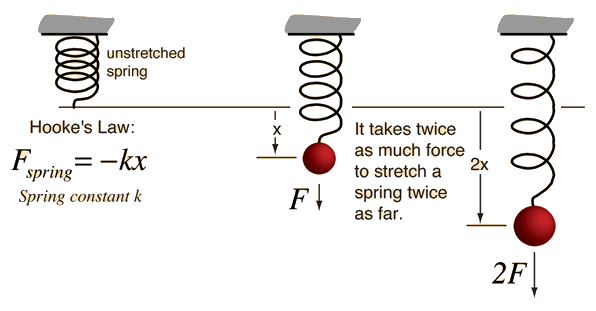
\includegraphics[width=8cm]{hooke.png}

In a play-area for children on the ferry there is a toy consisting of a mass attached to a spring hanging from the ceiling as shown in the figure above. Starting from the basic relation $F(x(t))=-kx(t)$, derive a general expression for the velocity of the mass as a function of time.




\subsubsection{4}

As you approach the port in Busan the engine of the ferry switches to reverse. During the switching, the casing of the engine vibrates with the motion described by this 2nd-order differential equation:
\begin{equation}
    3y''-4y'+y = t e^t
\end{equation}
The chief engineer wants to know the motion of the casing $y(t)$ as a function of time. Using the method of undetermined coefficients, find the general solution to this differential equation.




\newpage
\section{2016}
\subsection{Questions}
\subsubsection{1}

Solve the following ODE for $y$ given the condition $y(3)=9e^9$.

\begin{equation}
    \frac{x}{y} \frac{dy}{dx} - 1 = x^3
\end{equation}





\subsubsection{2}

The following equation is an autonamous equation:

\begin{equation}
    y'=\frac{y^2}{5}(1-\frac{y}{5})
\end{equation}
1. What key property does an autonamous equation have?


2. Determine the points of equilibrium and their stabilities.





\subsubsection{3}

Solve the following 2nd-order ODE's for $y$, and state what sort of damping they correspond to:

\begin{equation}
    y'' + 5 y' + 4y = 0 % Real
\end{equation}


\begin{equation}
    y'' + 4 y' + 4 y = 0 % Equal
\end{equation}


\begin{equation}
    y'' + 3 y' + 4 y = 0 % Complex
\end{equation}




\subsubsection{4}

Solve the following differential equation for $y$:

\begin{equation}
    3 x^2 y + 2 x y + y^3 + (x^2 + y^2) y' = 0
\end{equation}




\vspace{2cm}

\emph{Solutions can be found on the following page.}
\newpage

\subsection{Solutions}

\subsubsection{1}

$y=3xe^{x^3/3}$

\subsubsection{2}

1. $y'=f(y)$

2. $y=0$ (semi-stable), $y=5$ (stable)

\subsubsection{3}

$y(t)=C_1 e^{-t} + C_2 e^{-4t}$, Overdamped

$y(t)=C_1 e^{-2t} + C_2 t e^{-2t}$, Critically-damped

$y(t)=C_1 e^{-3t/2} Cos(\sqrt{7}t/2) + C_2 e^{-3t/2} Sin(\sqrt{7}t/2)$, Under-damped

\subsubsection{4}

$C = yx^2e^{3x} + \frac{1}{3} y^3 e^{3x}$


% Series solutions https://www.youtube.com/playlist?list=PLj7p5OoL6vGxVBxyLWLQHOCfFTIY_if5C
% Euler http://nbviewer.jupyter.org/github/engineersCode/EngComp/blob/master/modules/3_flyatchange/3_Get_Oscillations.ipynb
%       https://hub.mybinder.org/user/engineerscode-engcomp-7t4hdbpy/tree/modules/3_flyatchange 

\end{document}

% Interesting resources about the need for exponential and sinusoidal solutions
% https://www.youtube.com/watch?v=ZGPtPkTft8g (includes Laplace)
% https://math.stackexchange.com/questions/573581/why-is-the-formal-solution-to-a-linear-differential-equation-of-exponential-form
% https://math.stackexchange.com/questions/2502533/when-solving-a-differential-equation-why-do-we-always-start-with-guessing-the-s

